\chapter{软件测试与分析}

本章将展示软件的实现成果与测试情况,其中软件实现成果包含远端服务、边端服务、后台管理界面和电子秤模拟器四个部分,软件测试分为功能测试和性能测试两个部分。下面将首先给出软件的测试环境,然后对软件的功能和性能进行测试,同时对测试结果进行分析并得出相关结论。

\section{软件测试环境}

(1)测试环境:一台 8G 内存、8核 CPU 的 MacOS 系统。

(2)部署方式:按照图\ref{fig:软件部署架构图}中的部署架构,使用 Docker Compose 技术组织各个应用容器,采用本地部署的方式模拟远边端服务进行测试。如表\ref{tab:docker-compose}所示,第一列中显示了容器的名称,第二列显示了容器的具体描述。容器之间以桥接网络(Bridge)的形式进行通信。容器的名称作为网络别名,容器之间可以通过网络别名相互进行访问。

\begin{table}[H]
    \centering
    \caption{Docker Compose 应用容器组织情况}
    \label{tab:docker-compose}
\begin{tblr}
    {
    colspec        = {Q[c,m]X[l,m]},
    hline{1,Z}     = {wd=.08em},
    hline{2}       = {wd=.05em},
    row{even[2-Z]} = {bg=gray9!50},
    row{1}         = {font=\bfseries},
    rowhead        = 1,
    }
容器名称 & 容器描述 \\
mysql-server & 远端 MySQL 数据库服务  \\
mysql-edge & 边端 MySQL 数据库服务  \\
redis & 远端 Redis 缓存服务  \\
emqx1/emqx2/emqx3 & 边端 Emqx 静态集群  \\
minio-remote & 远端 Minio 对象存储服务  \\
minio-edge & 边端 Minio 对象存储服务  \\
minio-bucket-init & 远端 Minio 客户端初始化服务  \\
aws-edge & 边端 Spring Web 应用服务  \\
aws-server & 远端 Spring Web 应用服务  \\
aws-img & 远/边端 YOLO 图像识别服务  \\
aws-web & 远端 Vue 后台管理界面  \\
\end{tblr}
\end{table}

\section{软件功能测试}\label{sec:test-func}

下面将首先给出总体的测试结果,然后详细展示各个核心功能的测试结果。

根据功能需求汇总表\ref{tab:req-summary}中提到的功能,给出对应的测试结果,如表\ref{tab:test-req-summary}所示,列出了不同测试项的描述及测试结果,所有软件功能都已通过测试。

\begin{table}[H]
    \centering
    \caption{软件功能测试结果}
    \label{tab:test-req-summary}
\begin{tblr}
{
colspec        = {Q[c,m]X[l,m]},
hline{1,Z}     = {wd=.08em},
hline{2}       = {wd=.05em},
row{even[2-Z]} = {bg=gray9!50},
row{1}         = {font=\bfseries},
rowhead        = 1,
}
测试项 & 描述 & 测试结果 \\
电子秤管理 & 验证能否添加、编辑、查看电子秤 & 测试通过 \\
果实管理 & 验证能否添加、编辑、查看果实 & 测试通过 \\
作业管理 & 验证能否添加、编辑、查看作业 & 测试通过 \\
用户管理 & 验证能否添加、查看用户 & 测试通过 \\
称重记录处理 & 验证能否处理称重数据 & 测试通过 \\
待办记录处理 & 验证能否处理待办数据 & 测试通过 \\
称重历史获取 & 验证能否查看个人和电子秤称重历史 & 测试通过 \\
个人称重统计 & 验证能否查看和导出个人分作业批次采摘情况 & 测试通过 \\
果实称重统计 & 验证能否查看和导出果实分作业批次采摘情况和年产量情况 & 测试通过 \\
用户认证授权 & 验证能否认证和授权用户 & 测试通过 \\
果实图像识别 & 验证识别果实图像 & 测试通过 \\
果实图像存储 & 验证能否存储果实图像 & 测试通过  \\
远端和边端的数据同步 & 验证能否同步远端和边端数据 & 测试通过  \\
\end{tblr}
\end{table}

下面针对\ref{sec:req1}给出的核心需求用例分别进行详细的用例测试。

对提交称重数据需求用例\ref{tab:uc-weigh-submit}设计测试用例并进行测试,如表\ref{tab:uc-weigh-submit-test}所示,测试用例包括通过不同协议(如MQTT、CoAP、STOMP、HTTP)提交正常数据以及提交包含错误(如不存在的电子秤、果实、作业等)的异常数据。预期结果和实际结果都一致,正常数据提交返回“成功”,异常数据提交返回“失败”。

实际界面的测试结果如图\ref{fig:scale-simulator}所示。图中显示的是电子秤模拟器界面,包含9个输入框、4个操作按钮和1个结果显示区。其中输入框包含通信协议(MQTT、HTTP、STOMP、CoAP)、电子秤编号、员工编号、果实编号、果实名称、果实图片、重量值、误差值和单位;提交按钮包含识别果实按钮、生成数据按钮、提交数据按钮和清除结果按钮;结果显示区包含记录编号、通信协议、作业编号、果实编号和提交结果。

\begin{table}[H]
    \centering
    \caption{提交称重数据用例测试}
    \label{tab:uc-weigh-submit-test}
\begin{tblr}
{
    colspec={Q[c,m]X[c,m]},
    hlines,vlines,cell{2-Z}{1}={},
    cell{1-Z}{1}={font=\bfseries},
    cell{1-Z}{2}={halign=l}
}
用例名称 & 提交称重数据 \\

用例描述 & 采摘员工在电子秤提交称重数据 \\

用例入口 & 电子秤提交称重数据 \\

测试步骤 & 步骤1. 运行电子秤模拟器\newline
步骤2. 点击生成数据\newline
步骤3. 点击识别果实\newline
步骤4. 点击提交数据 \\

测试用例 & 用例1: 通过 MQTT 协议提交正常数据\newline
用例2: 通过 CoAP 协议提交正常数据\newline
用例3: 通过 STOMP 协议提交正常数据\newline
用例4: 通过 HTTP 协议提交正常数据\newline
用例5: 通过 MQTT 协议提交异常数据(不存在的电子秤, 编号为999)\newline
用例6: 通过 MQTT 协议提交异常数据(未启用的电子秤, 电子秤编号为1)\newline
用例7: 通过 MQTT 协议提交异常数据(不存在的果实, 果实编号为999)\newline
用例8: 通过 MQTT 协议提交异常数据(未启用的果实, 果实编号为1)\newline
用例9: 通过 MQTT 协议提交异常数据(不存在的采摘作业,果实编号为3)\newline
用例10: 通过 MQTT 协议提交异常数据(未开始或已结束的采摘作业,作业编号为4) \\

预期结果与实际结果 & 用例1-5:预期返回"成功",实际结果一致\newline
用例6-10:预期返回"失败",实际结果一致\\

\end{tblr}
\end{table}

\begin{figure}
    \centering
    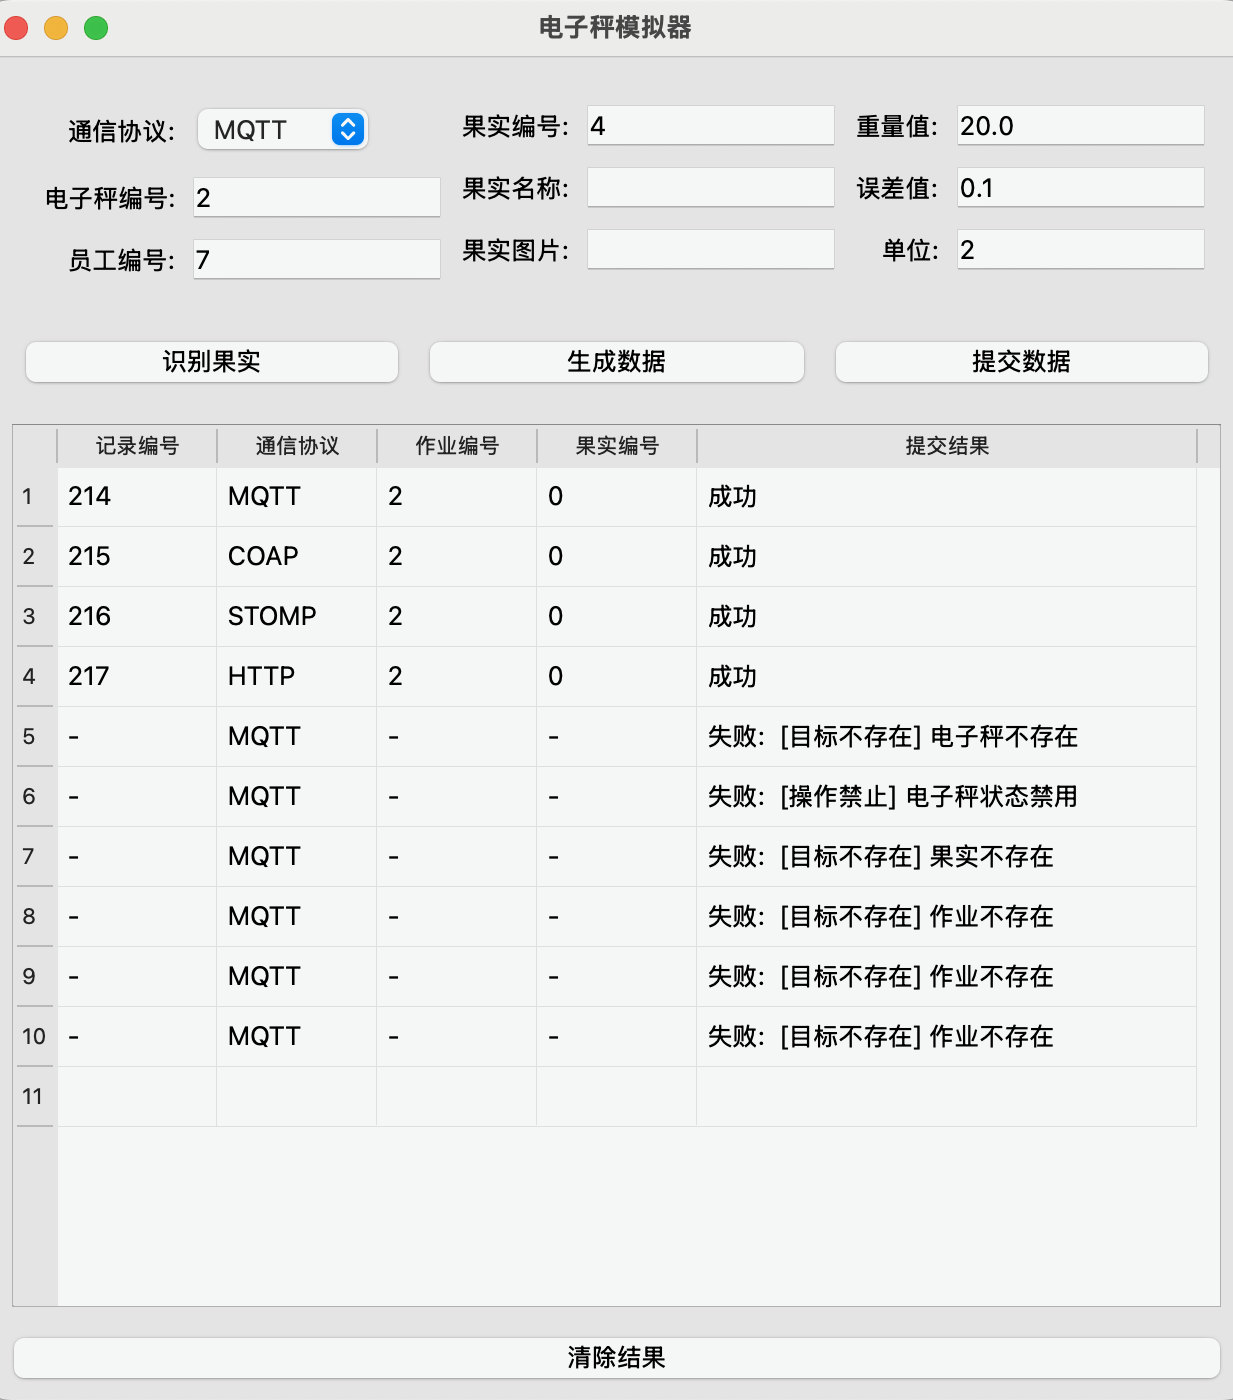
\includegraphics[width=0.9\linewidth]{../result/scale-simulator.png}
    \caption{电子秤模拟器界面}
    \label{fig:scale-simulator}
\end{figure}

对处理待办记录需求用例\ref{tab:uc-todo-handle}设计测试用例并进行测试,如表\ref{tab:uc-todo-handle-test}所示,测试用例包括提交正常数据和异常数据(如不存在的果实或未启用的果实)。测试步骤涵盖点击提交待办、选择果实种类并完成待办的操作。预期结果与实际结果一致,正常数据提交返回“成功”,而异常数据提交则返回“失败”。

实际界面的测试情况如图\ref{fig:web-todo}和图\ref{fig:form-todo-handle}所示。图\ref{fig:web-todo}展现了软件管理后台中的待办管理界面,其中包含操作面板、待办列表和分页块。操作面板包含四个操作按钮,分别是提交、丢弃、批量提交和批量丢弃。待办列表表头包含编号、果实编号、果实名称、果实图像、员工编号、电子秤编号、称重数据、误差、称重时间和支持的操作项,其中操作项包含提交和丢弃。

对某个待办项,点击提交按钮后,显示表单如图\ref{fig:form-todo-handle}所示,包含2个操作按钮和9个表单项,其中操作按钮包含取消和确认按钮;表单项包含选择果实、果实名称、果实编号、果实图像、员工编号、电子秤编号、称重数据、误差、称重时间,其中只能编辑果实,从选择果实项的下滑表单中选择果实后,果实名称和果实编号项将会随之变化。

\begin{table}
    \centering
    \caption{处理待办记录用例测试}
    \label{tab:uc-todo-handle-test}
\begin{tblr}
    {
        colspec={Q[c,m]X[c,m]},
        hlines,vlines,cell{2-Z}{1}={},
        cell{1-Z}{1}={font=\bfseries},
        cell{1-Z}{2}={halign=l}
    }
用例名称 & 处理待办记录 \\

用例描述 & 管理员在管理后台界面处理待办记录 \\

用例入口 & 后台管理界面中的待办管理模块 \\

测试步骤 & 步骤1. 点击提交待办 \newline
步骤2. 选择果实种类 \newline
步骤3. 点击确定,完成待办 \\

测试用例 & 用例1: 提交正常数据 \newline
用例2: 提交异常数据(不存在的果实, 果实编号为999) \newline
用例3: 提交异常数据(未启用的果实, 果实编号为1) \\

预期结果与实际结果 & 用例1:预期返回"成功",实际结果一致 \newline
用例2:预期返回"失败",实际结果一致 \newline
用例3:预期返回"失败",实际结果一致 \\

\end{tblr}
\end{table}

\begin{figure}
    \centering
    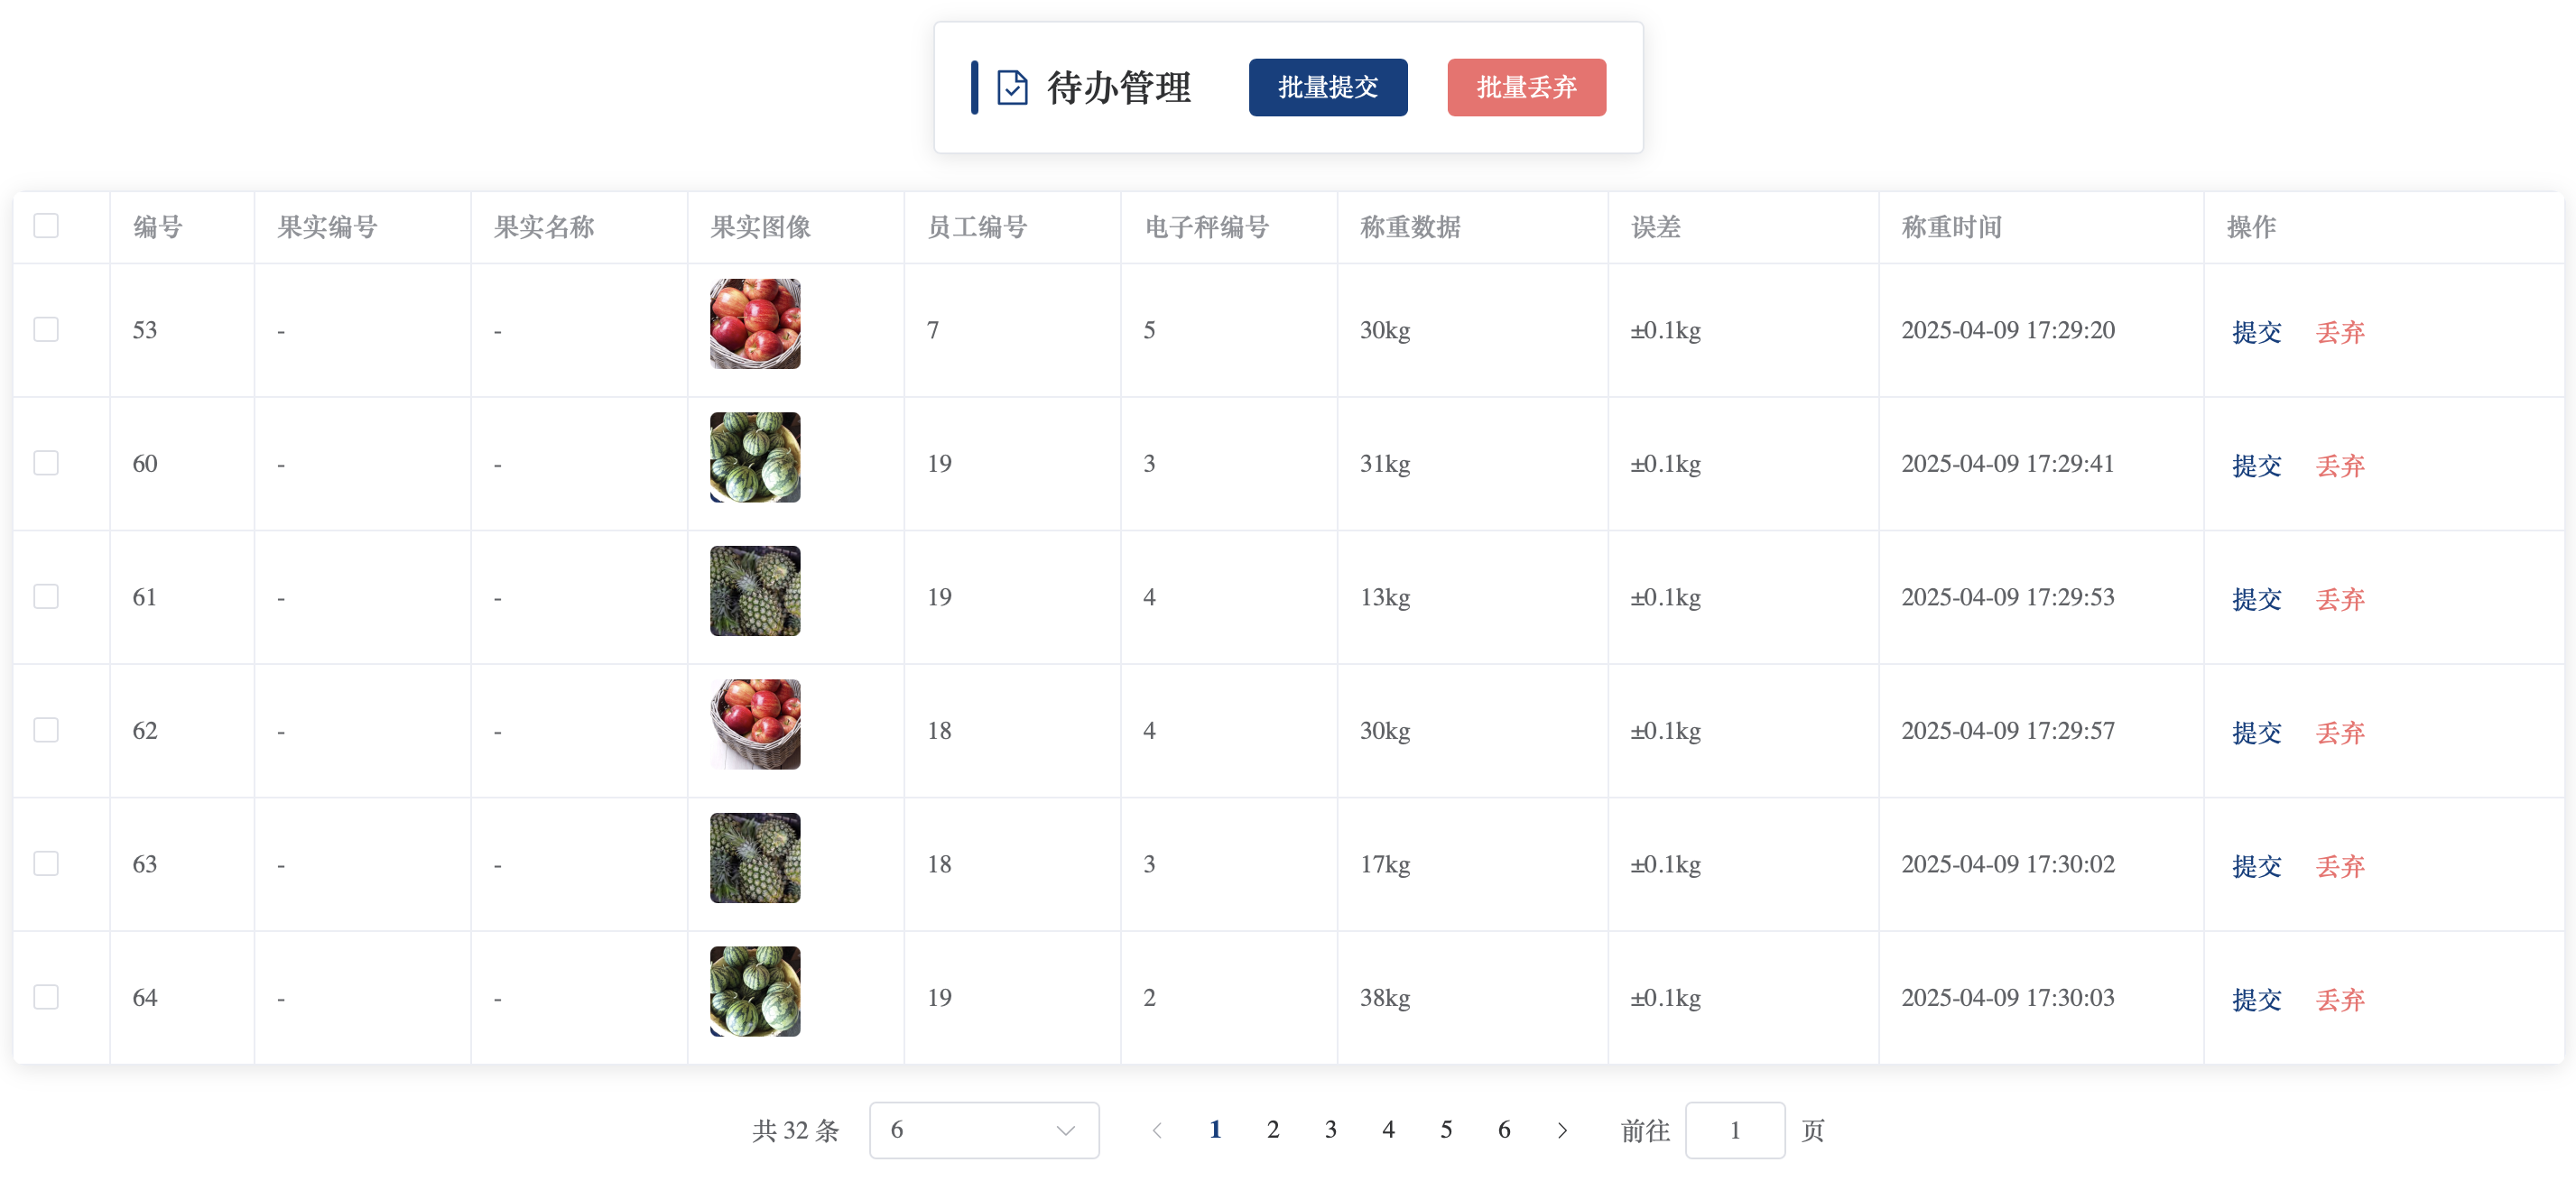
\includegraphics[width=0.9\linewidth]{../result/web-todo.png}
    \caption{待办管理界面}
    \label{fig:web-todo}
\end{figure}

\begin{figure}
    \centering
    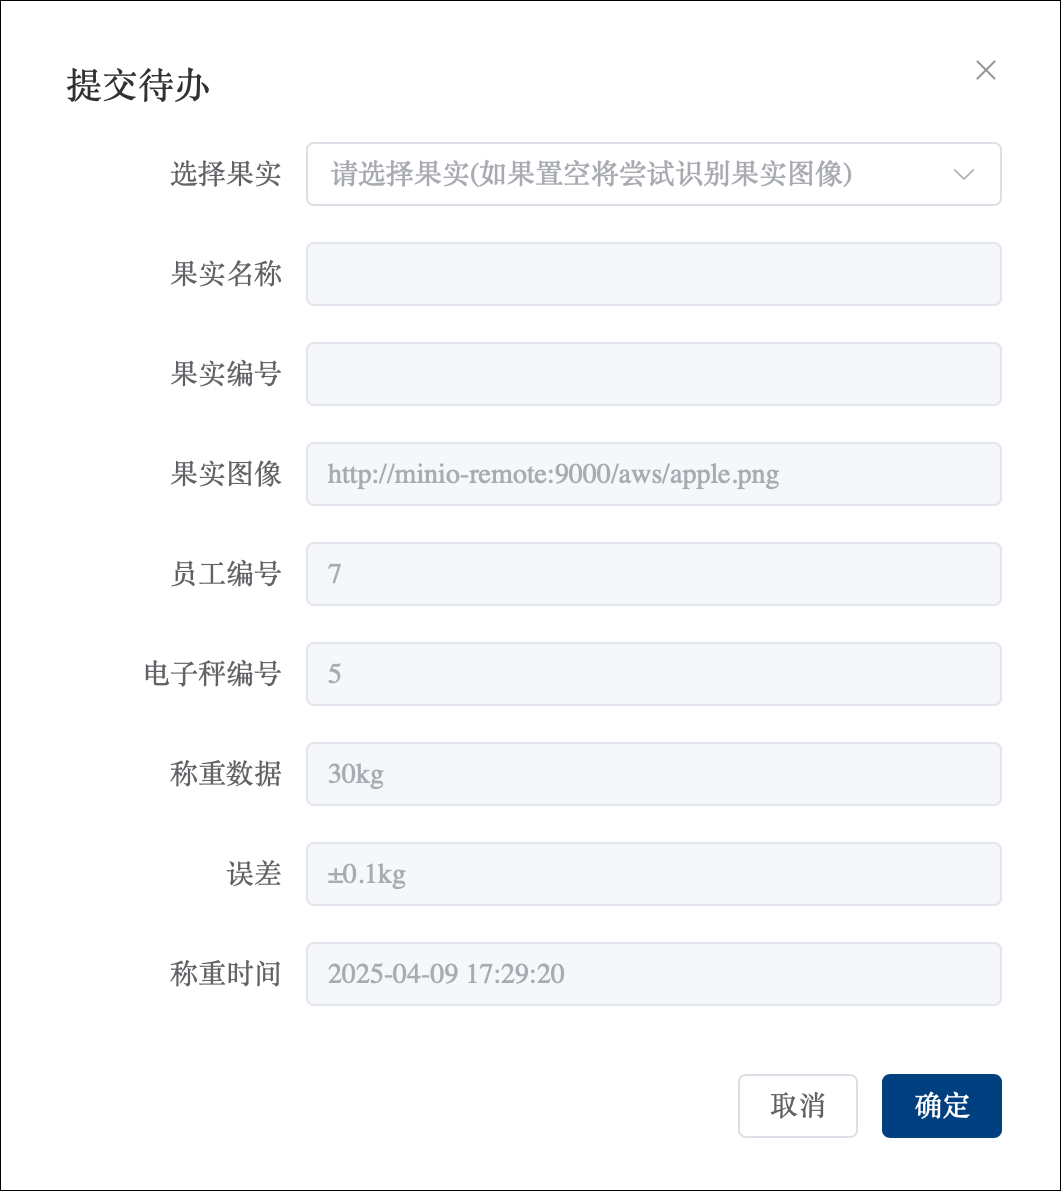
\includegraphics[height=0.5\textheight]{../result/form-todo-handle.png}
    \caption{提交待办表单}
    \label{fig:form-todo-handle}
\end{figure}

对称重记录统计分析需求用例\ref{tab:uc-record-analysis}设计测试用例并进行测试,如表\ref{tab:uc-record-analysis-test}所示,测试用例涉及查看苹果的年产量、分批产量以及查看特定用户的分批产量,并导出为Excel。预期结果和实际结果一致,分别得到了折线图、统计结果表格以及对应的Excel表格。

实际界面的测试情况如图\ref{fig:web-produce}、图\ref{fig:chart-apple-year}、图\ref{fig:chart-apple-works}、图\ref{fig:web-me}、图\ref{fig:chart-user-works}、图\ref{fig:chart-excels}所示。

\begin{table}
    \centering
    \caption{称重记录统计分析用例测试}
    \label{tab:uc-record-analysis-test}
\begin{tblr}
    {
        colspec={Q[c,m]X[c,m]},
        hlines,vlines,cell{2-Z}{1}={},
        cell{1-Z}{1}={font=\bfseries},
        cell{1-Z}{2}={halign=l}
    }

用例名称 & 称重记录统计分析 \\

用例描述 & 在管理后台界面查看果实和采摘人员的称重记录统计情况 \\

用例入口 & 后台管理界面中的果实/用户管理模块 \\

测试步骤 & 步骤1. 管理员访问果实/用户管理界面 \newline
步骤2. 管理员点击某个可视化选项进行查看并导出 \\

测试用例 & 用例1:点击查看苹果的年产量并导出为 Excel \newline
用例2: 点击查看苹果的分批产量并导出为 Excel \newline
用例3: 点击查看用户(用户编号为3)的分批产量并导出为 Excel  \\

预期结果与实际结果 & 用例1:预期得到折线图和对应的 Excel 表格,实际结果一致 \newline
用例2:预期得到折线图和对应的 Excel 表格,实际结果一致 \newline
用例3:预期得到统计结果表格和对应的 Excel 表格,实际结果一致 \\

\end{tblr}
\end{table}

访问果实管理界面,得到如图\ref{fig:web-produce}的结果。果实管理界面包含了操作面板、果实列表和分页块。操作面板包含四个操作按钮,分别是添加果实、查询果实、导出所有果实年产量数据和导出所有果实分批产量数据。果实列表表头包含编号、名称、状态、创建时间、更新时间和支持的操作项,其中操作项包含查看年产量、分批产量和编辑操作。

\begin{figure}
    \centering
    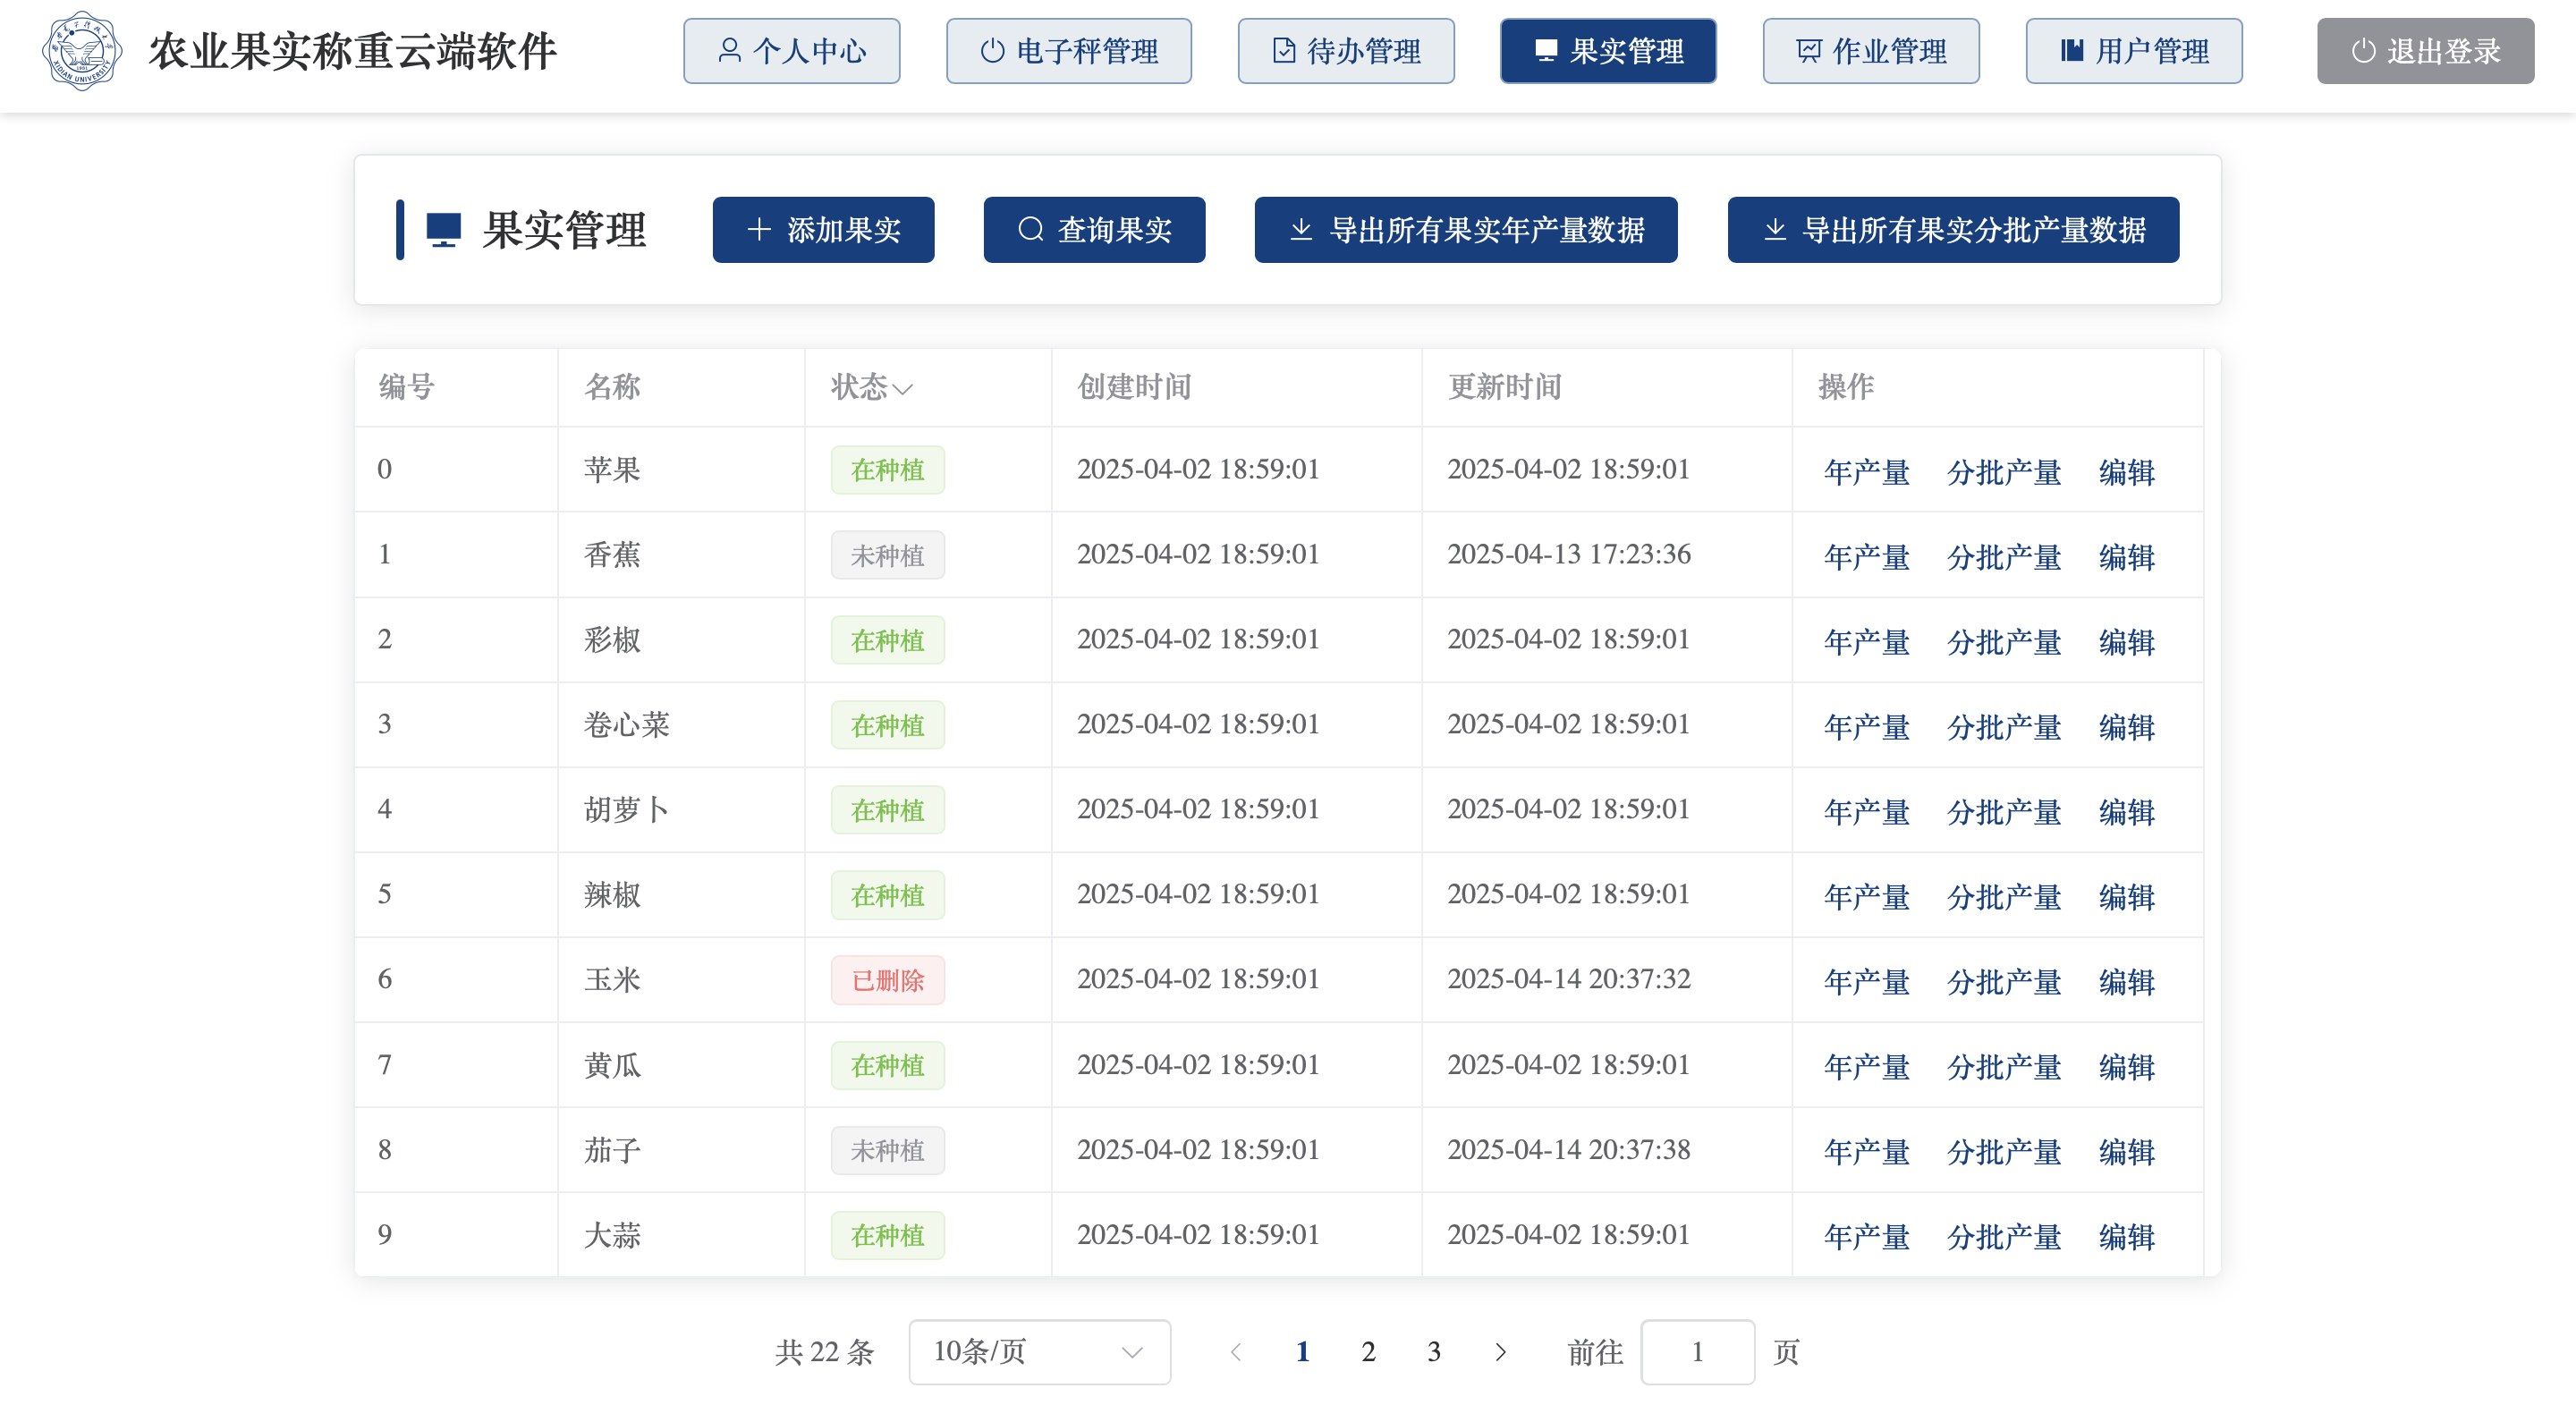
\includegraphics[width=0.9\linewidth]{../result/web-produce.png}
    \caption{果实管理界面}
    \label{fig:web-produce}
\end{figure}

\begin{figure}[H]
    \centering
    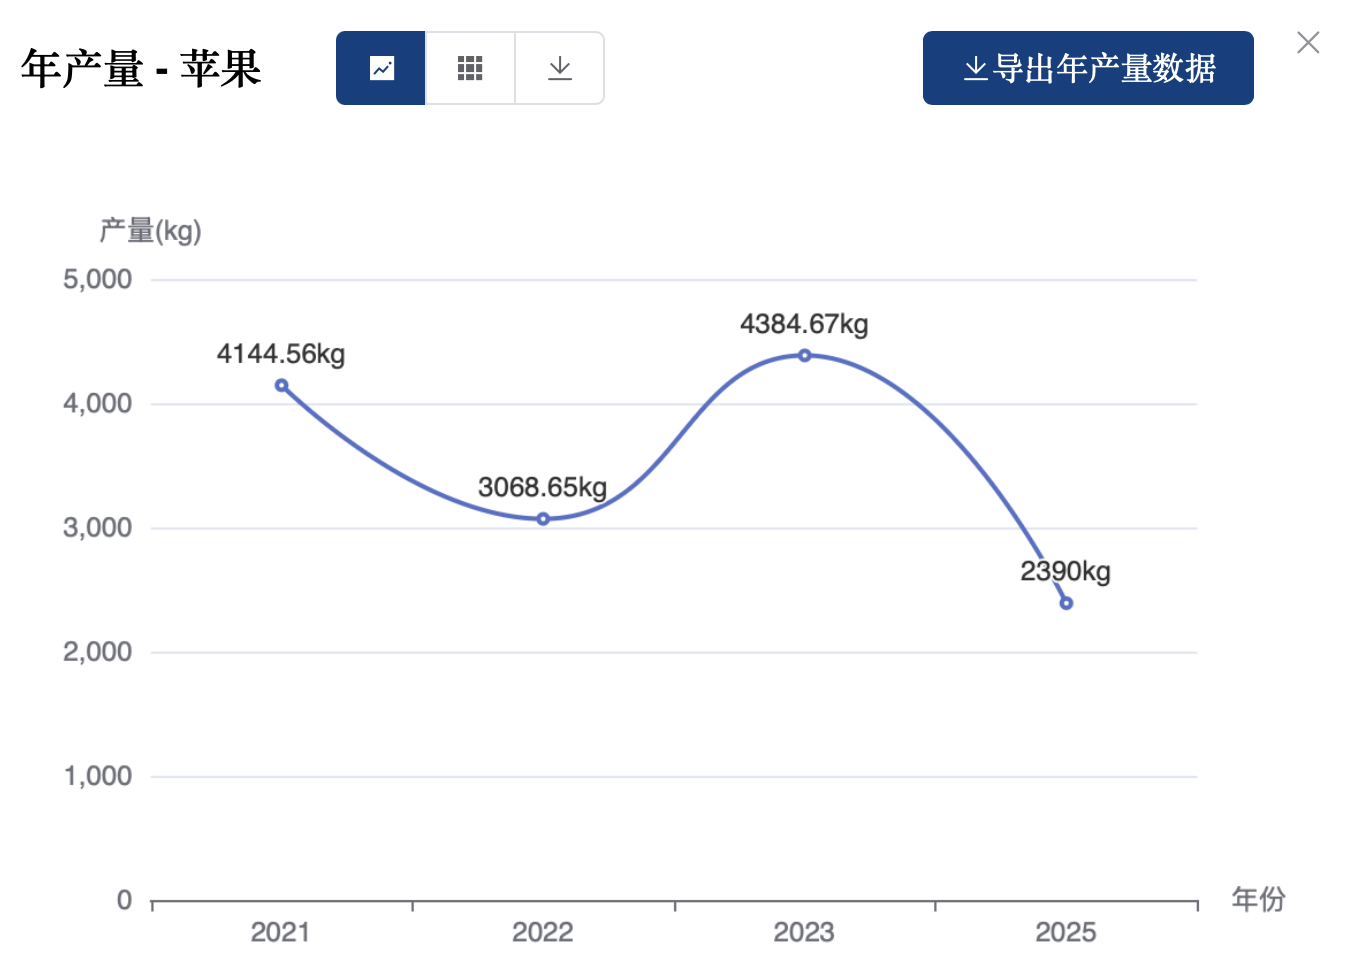
\includegraphics[width=0.9\linewidth]{../result/chart-apple-year.png}
    \caption{苹果年产量折线图}
    \label{fig:chart-apple-year}
\end{figure}

在果实管理界面中,对果实列表中的苹果条目,点击年产量操作按钮,得到如图\ref{fig:chart-apple-year}所示的苹果年产量,折线图中横坐标为年份,纵坐标为产量(kg);点击分批产量操作按钮,得到如图\ref{fig:chart-apple-works}所示的苹果分批产量,折线图中横坐标为作业编号,纵坐标为产量(kg)。

\begin{figure}[H]
    \centering
    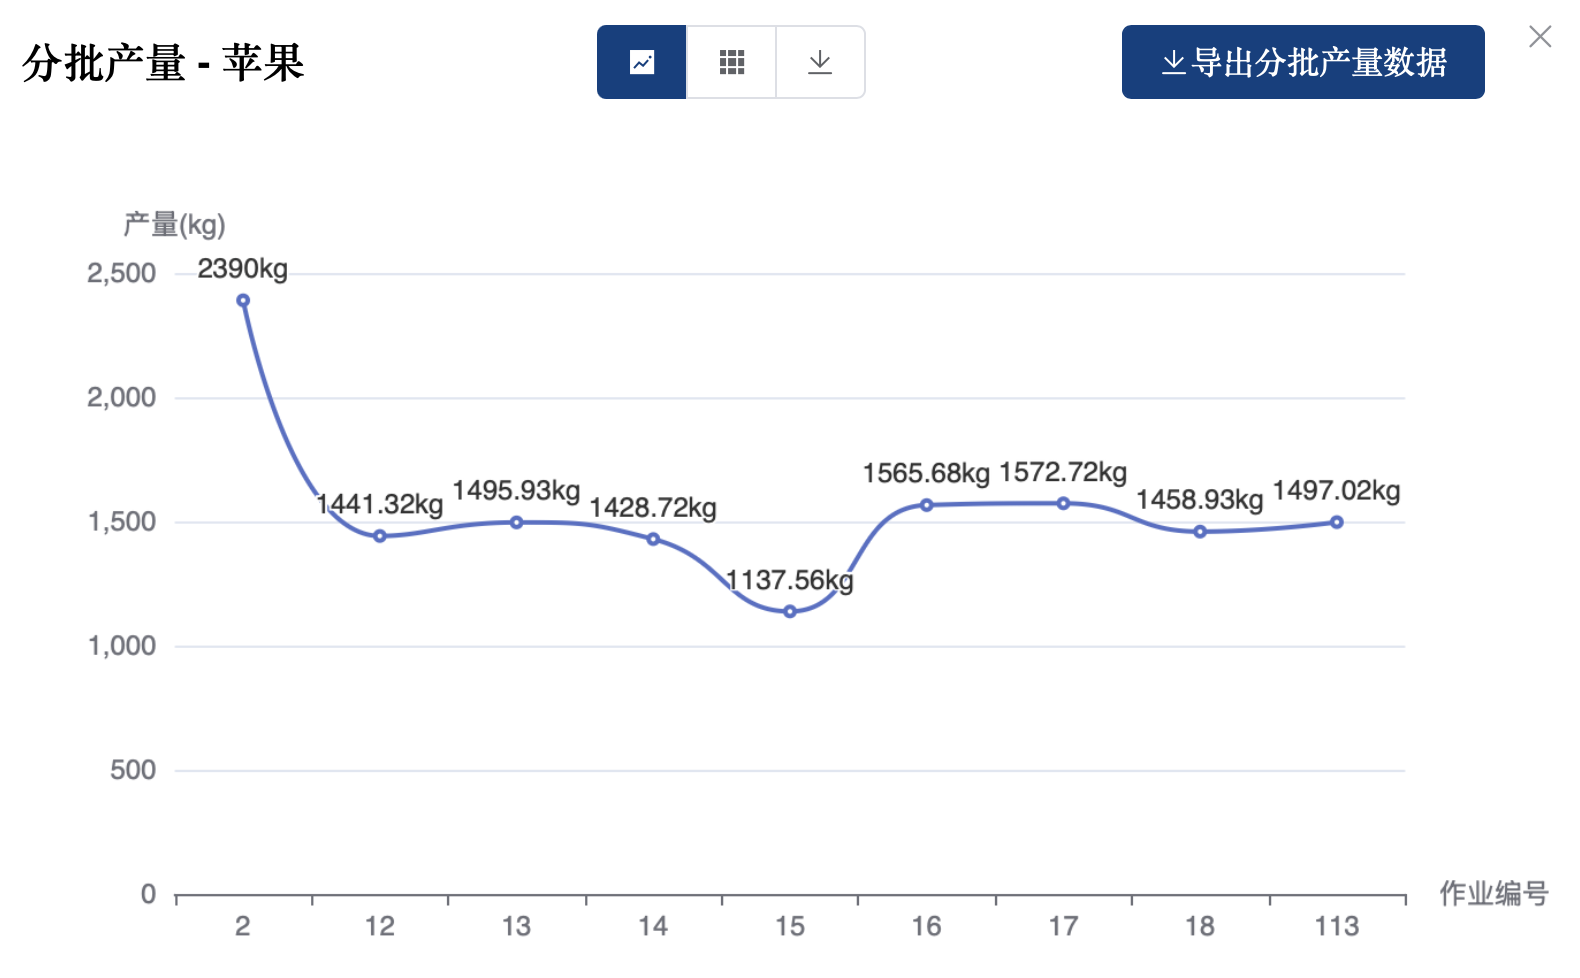
\includegraphics[width=0.9\linewidth]{../result/chart-apple-works.png}
    \caption{苹果分批产量折线图}
    \label{fig:chart-apple-works}
\end{figure}

访问个人中心界面,得到如图\ref{fig:web-me}的结果。个人中心界面包含了操作面板和个人信息。操作面板包含三个操作按钮,分别是编辑个人信息、查看个人称重历史和查看个人分批次采摘量。个人信息中包含了员工编号、身份证号、名称、角色和入职时间。

\begin{figure}
    \centering
    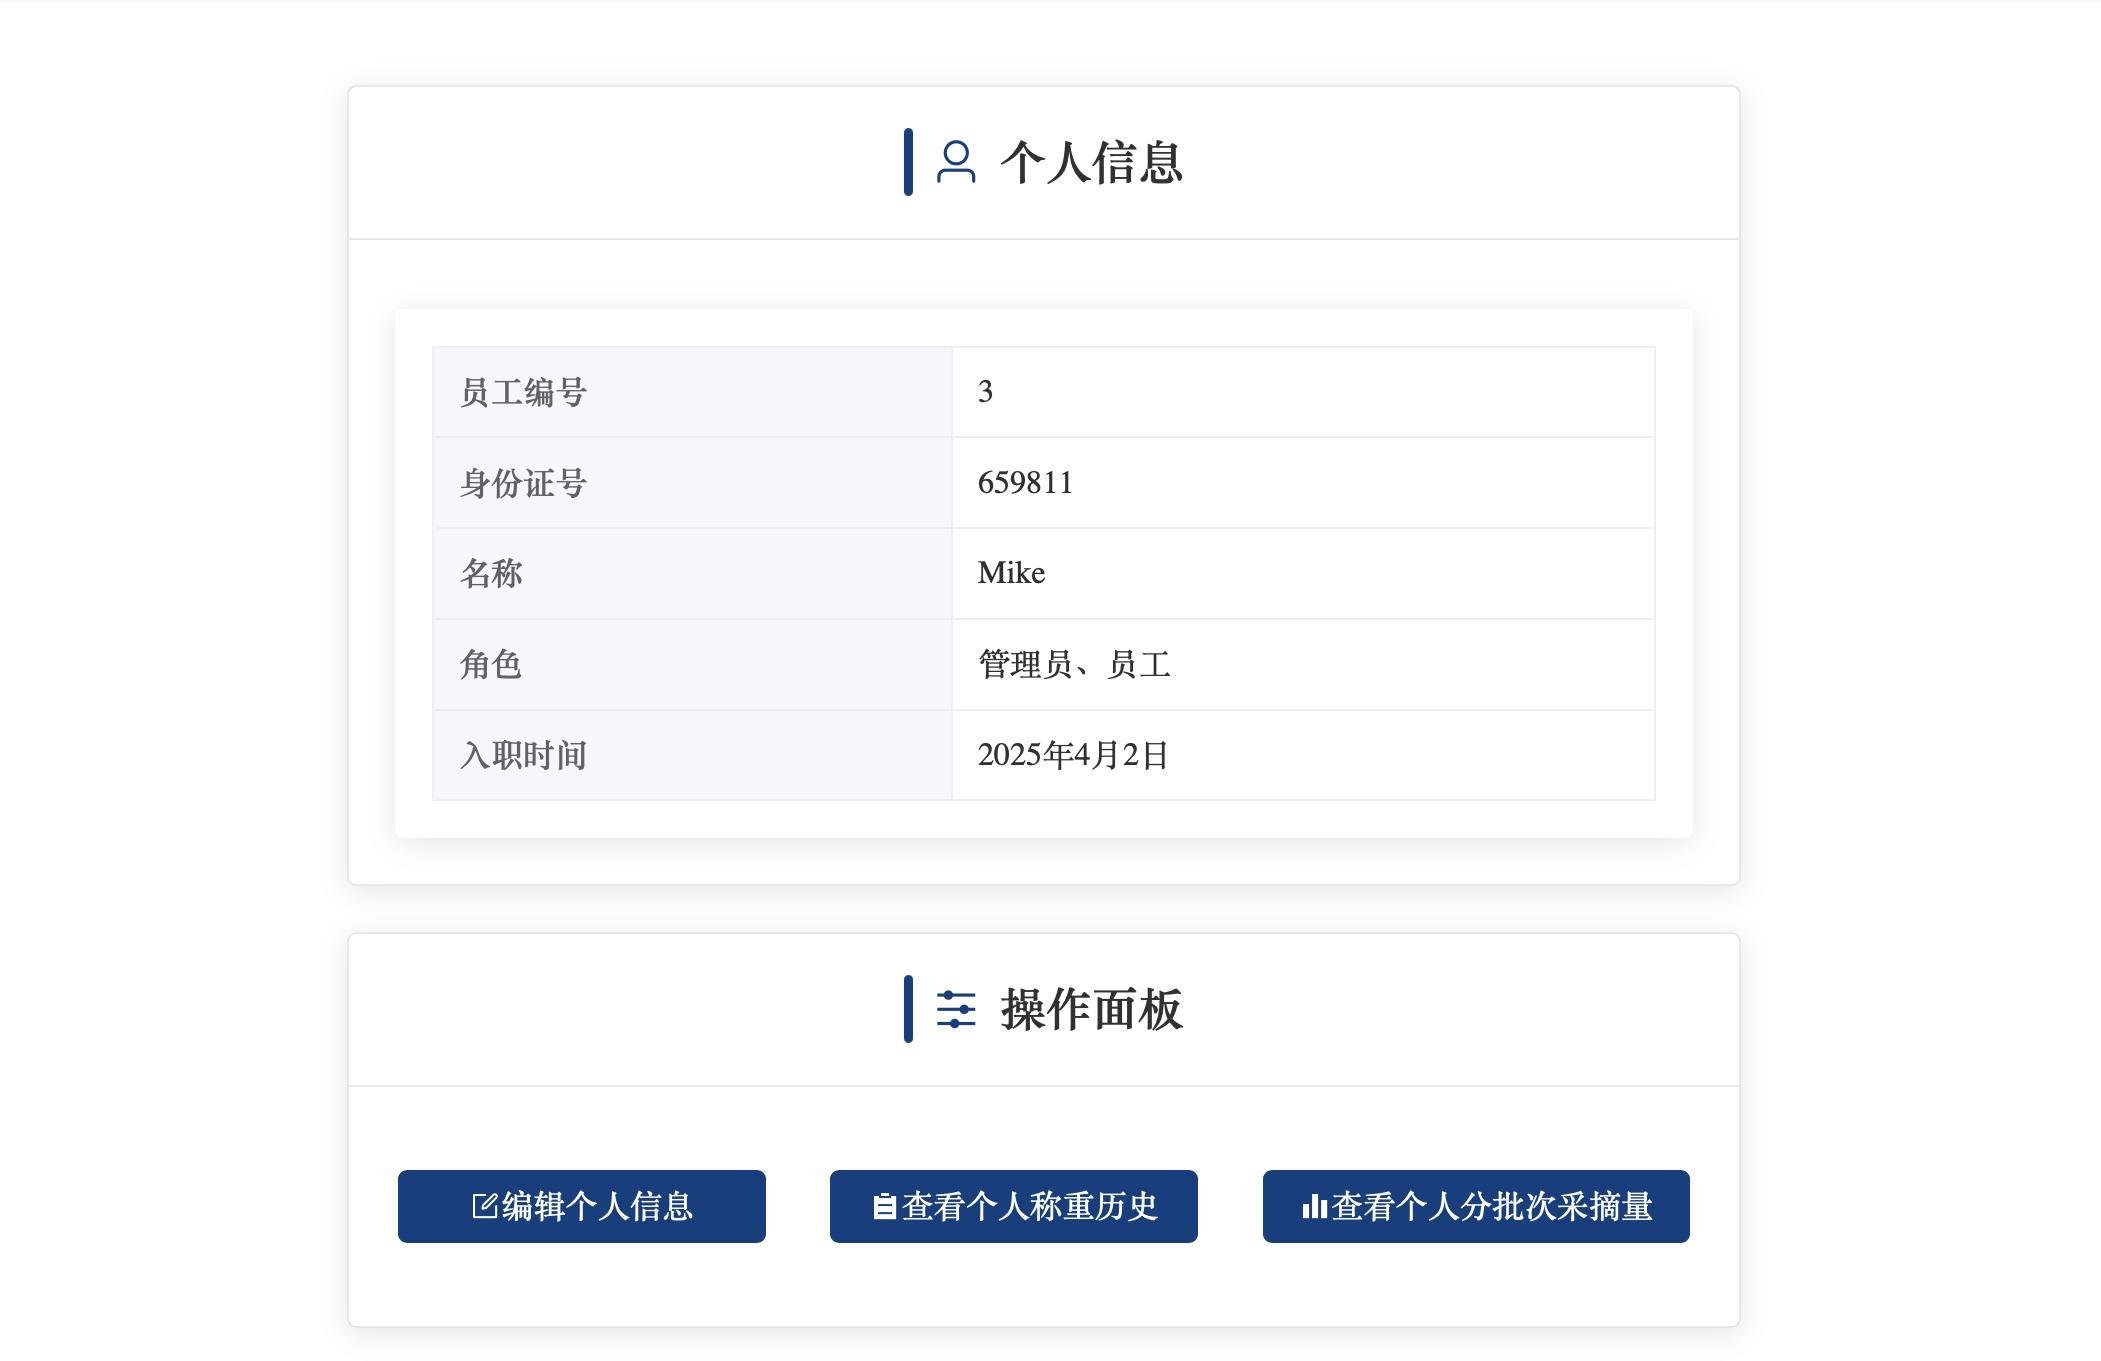
\includegraphics[width=0.9\linewidth]{../result/web-me.png}
    \caption{个人中心界面}
    \label{fig:web-me}
\end{figure}

访问用户管理界面,得到如图\ref{fig:web-user}的结果。用户管理界面包含了操作面板、用户列表和分页块。操作面板包含两个操作按钮,分别是添加用户按钮和查询用户按钮。用户列表表头从左到右分别是编号、身份证号、姓名、角色、状态、创建时间和支持的操作项,操作项包含查看称重历史、查看分批采摘量以及编辑操作。

\begin{figure}
    \centering
    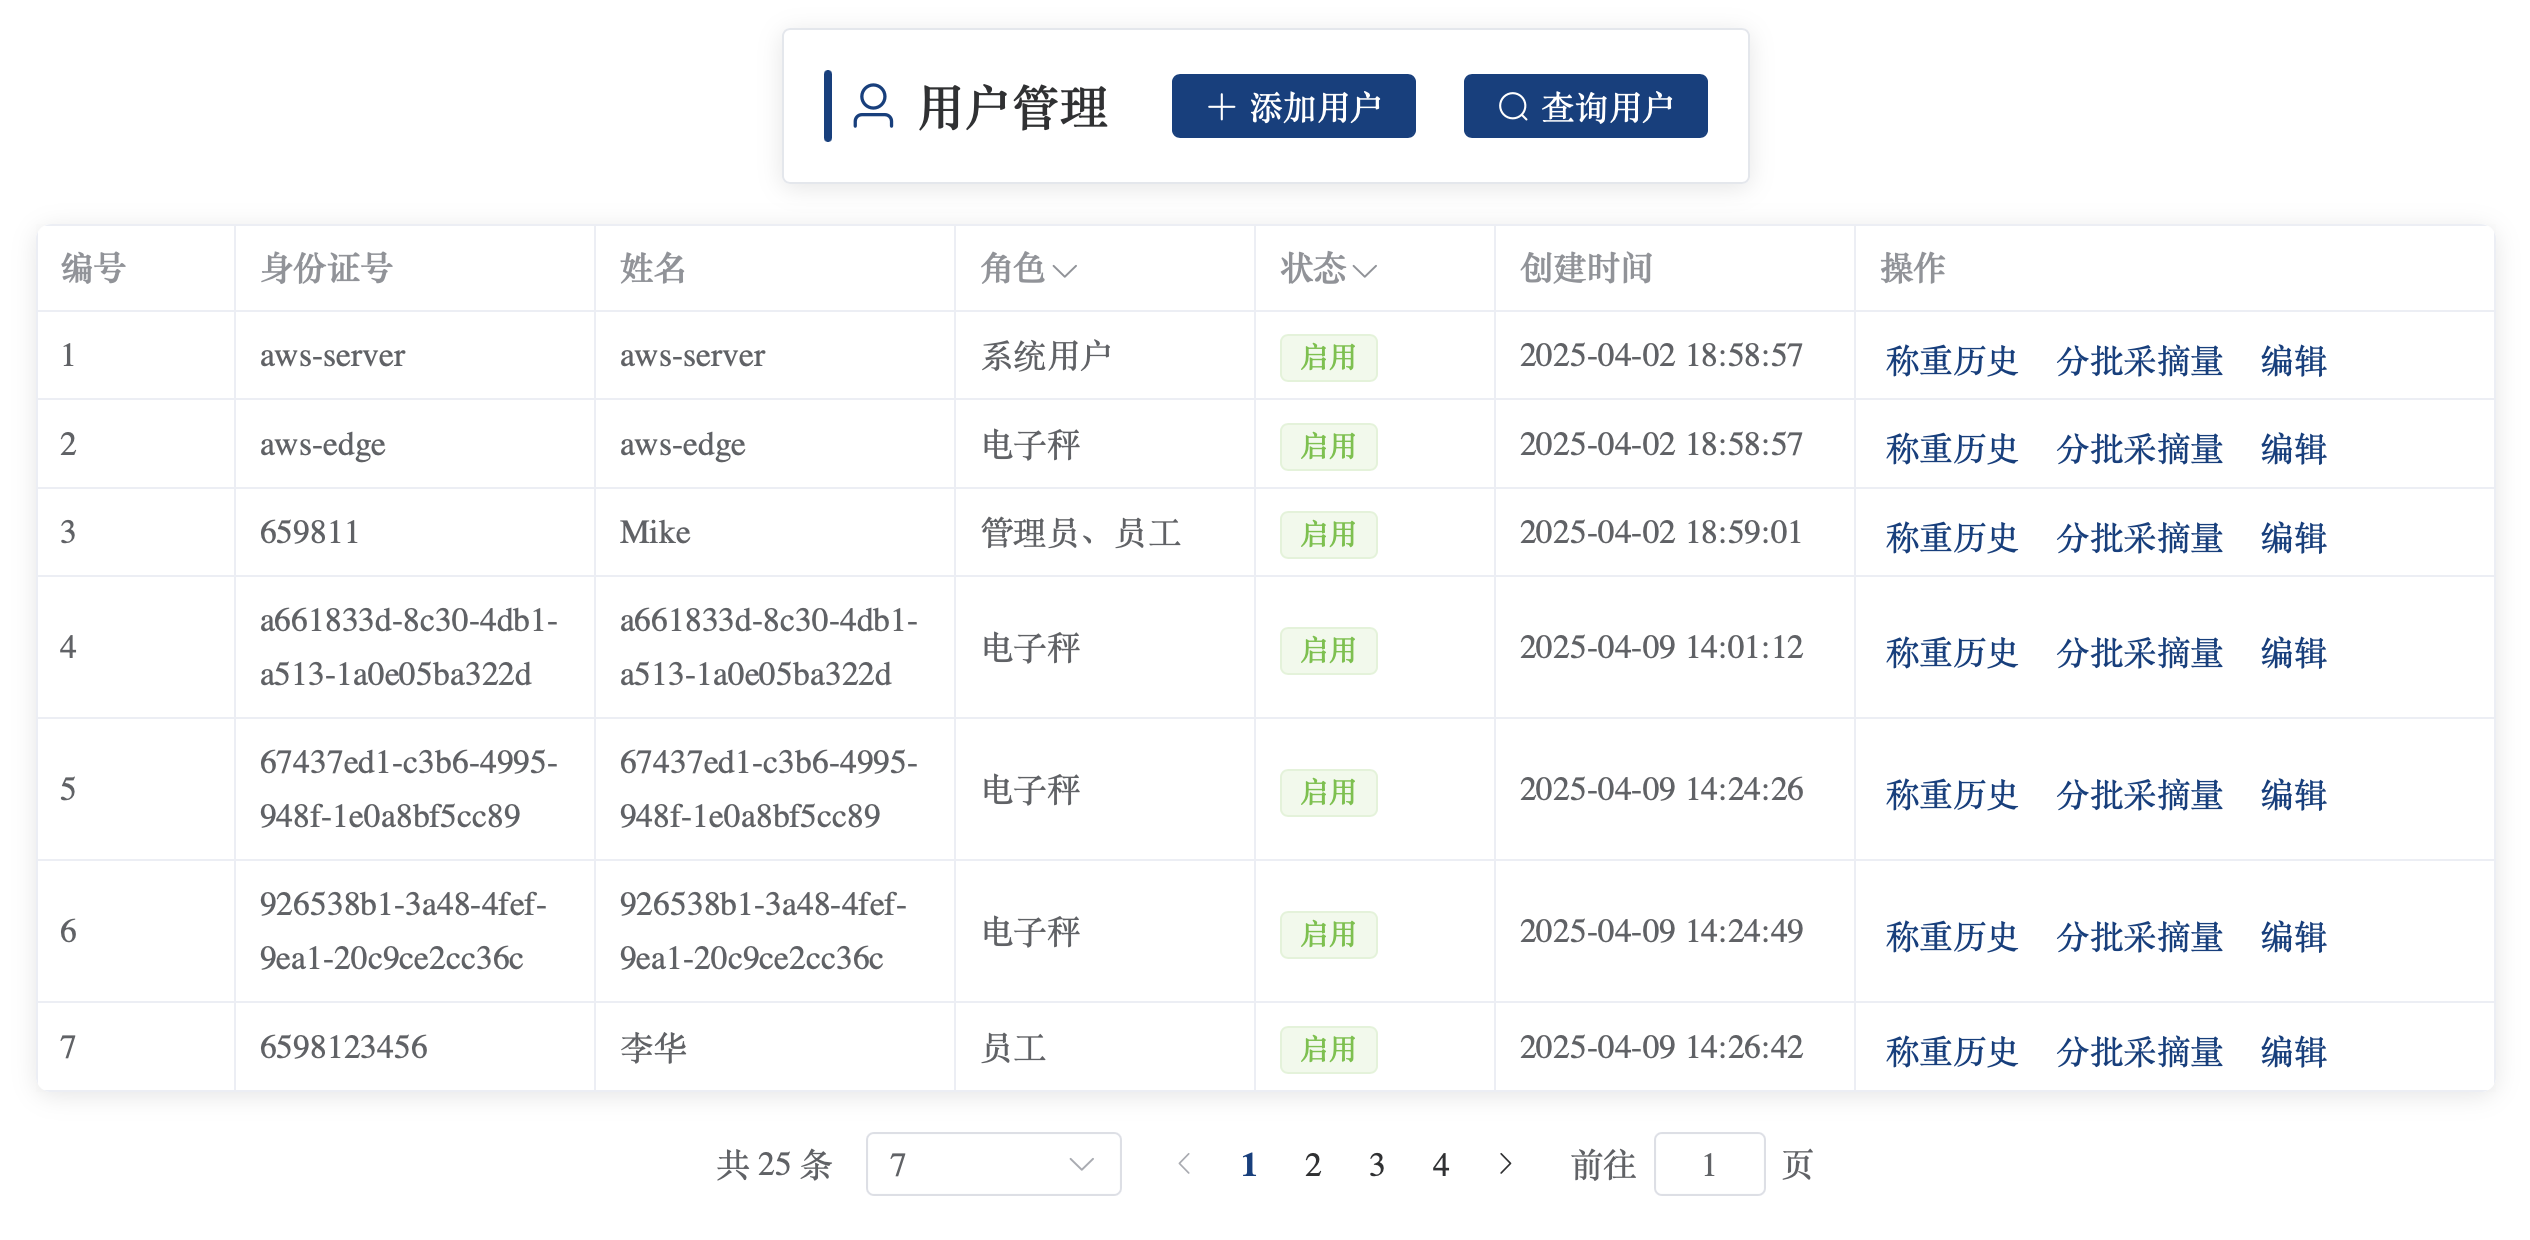
\includegraphics[width=0.9\linewidth]{../result/web-user.png}
    \caption{用户管理界面}
    \label{fig:web-user}
\end{figure}

在个人中心界面或用户管理界面中,点击查看分批次采摘量按钮,得到如图\ref{fig:chart-user-works}所示的员工分批采摘量,其中表头包含作业编号、果实名称和采摘量。

\begin{figure}
    \centering
    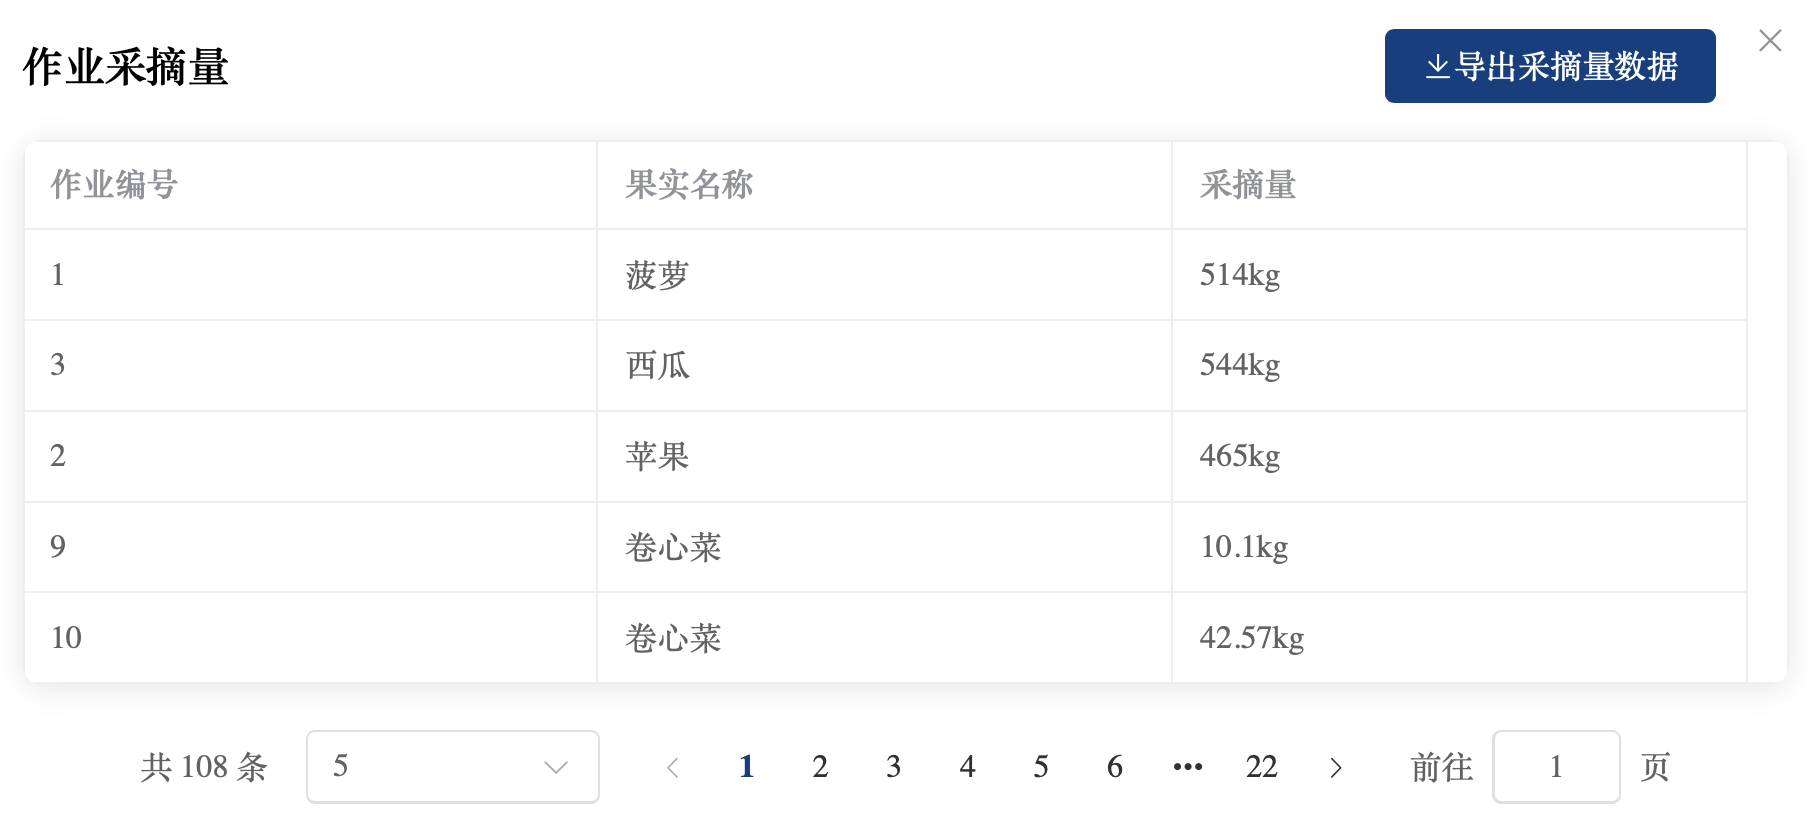
\includegraphics[width=0.9\linewidth]{../result/chart-user-works.png}
    \caption{员工分批采摘量表格}
    \label{fig:chart-user-works}
\end{figure}

每个可视化图表都支持导出,点击图表右上方的导出按钮即可将统计结果导出为 Excel,图\ref{fig:chart-excels}展现了前面三个图表导出的结果,从左至右分别展现了果实的年产量表格、果实的分批产量表格和员工的分批采摘量表格。

\begin{figure}
    \centering
    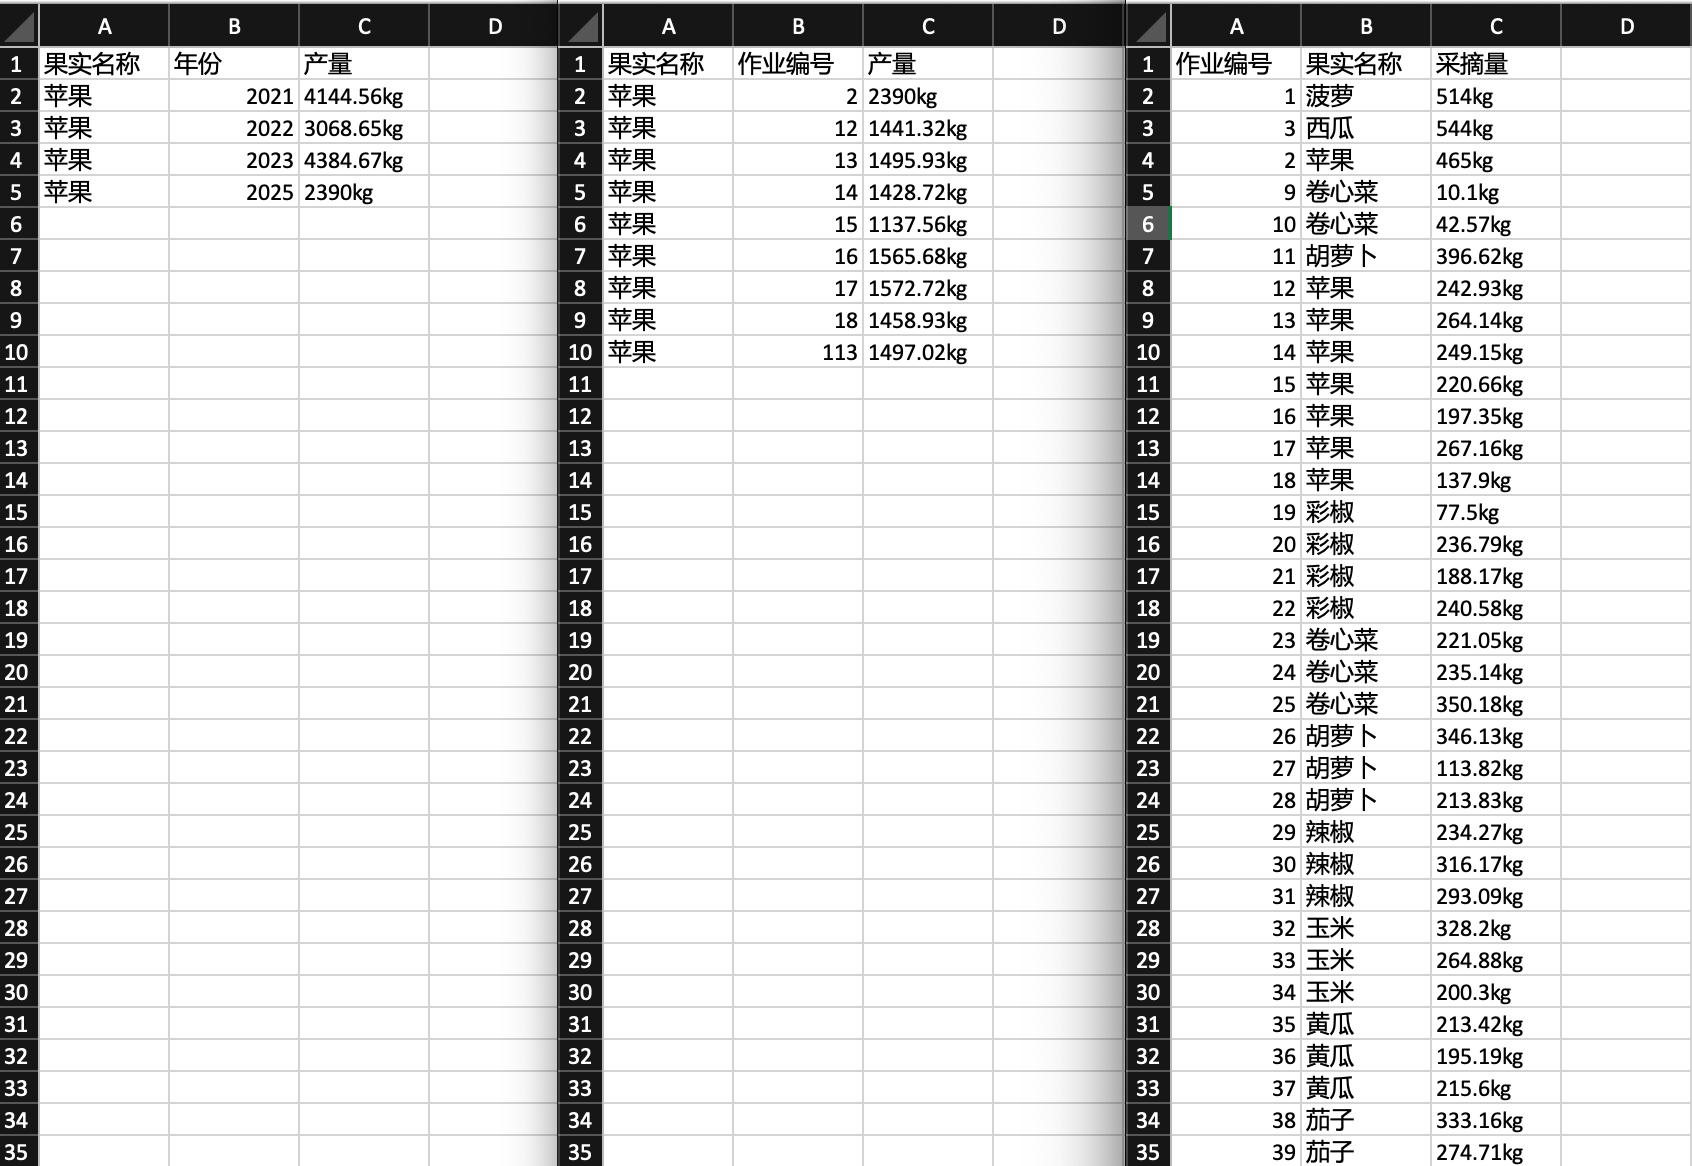
\includegraphics[width=0.9\linewidth]{../result/chart-excels.png}
    \caption{Excel 导出结果}
    \label{fig:chart-excels}
\end{figure}

对配置电子秤需求用例\ref{tab:uc-config-scale}设计测试用例并进行测试,如表\ref{tab:uc-config-scale-test}所示,测试用例包括提交完整信息的电子秤和缺少关键信息的电子秤。预期结果与实际结果一致,成功提交完整信息的电子秤时返回”成功”,缺失信息时返回”失败”。

\begin{table}[H]
    \centering
    \caption{配置电子秤用例测试}
    \label{tab:uc-config-scale-test}
\begin{tblr}
    {
        colspec={Q[c,m]X[c,m]},
        hlines,vlines,cell{2-Z}{1}={},
        cell{1-Z}{1}={font=\bfseries},
        cell{1-Z}{2}={halign=l}
    }

用例名称 & 配置电子秤 \\

用例描述 & 在管理后台界面配置并添加电子秤,将电子秤接入云端 \\

用例入口 & 后台管理界面中的电子秤管理模块 \\

测试步骤 & 步骤1. 管理员访问电子秤管理界面 \newline
步骤2. 管理员点击添加电子秤按钮 \newline
步骤3. 管理员编辑电子秤配置并提交 \\

测试用例 & 用例1:提交信息完整的电子秤 \newline
用例2: 提交信息有遗漏的电子秤(缺失密钥/型号) \\

预期结果与实际结果 & 用例1:预期返回"成功",实际结果一致 \newline
用例2:预期返回"失败",实际结果一致 \\

\end{tblr}
\end{table}

实际界面的测试结果如图\ref{fig:web-scale}和图\ref{fig:form-new-scale}所示。

\begin{figure}[H]
    \centering
    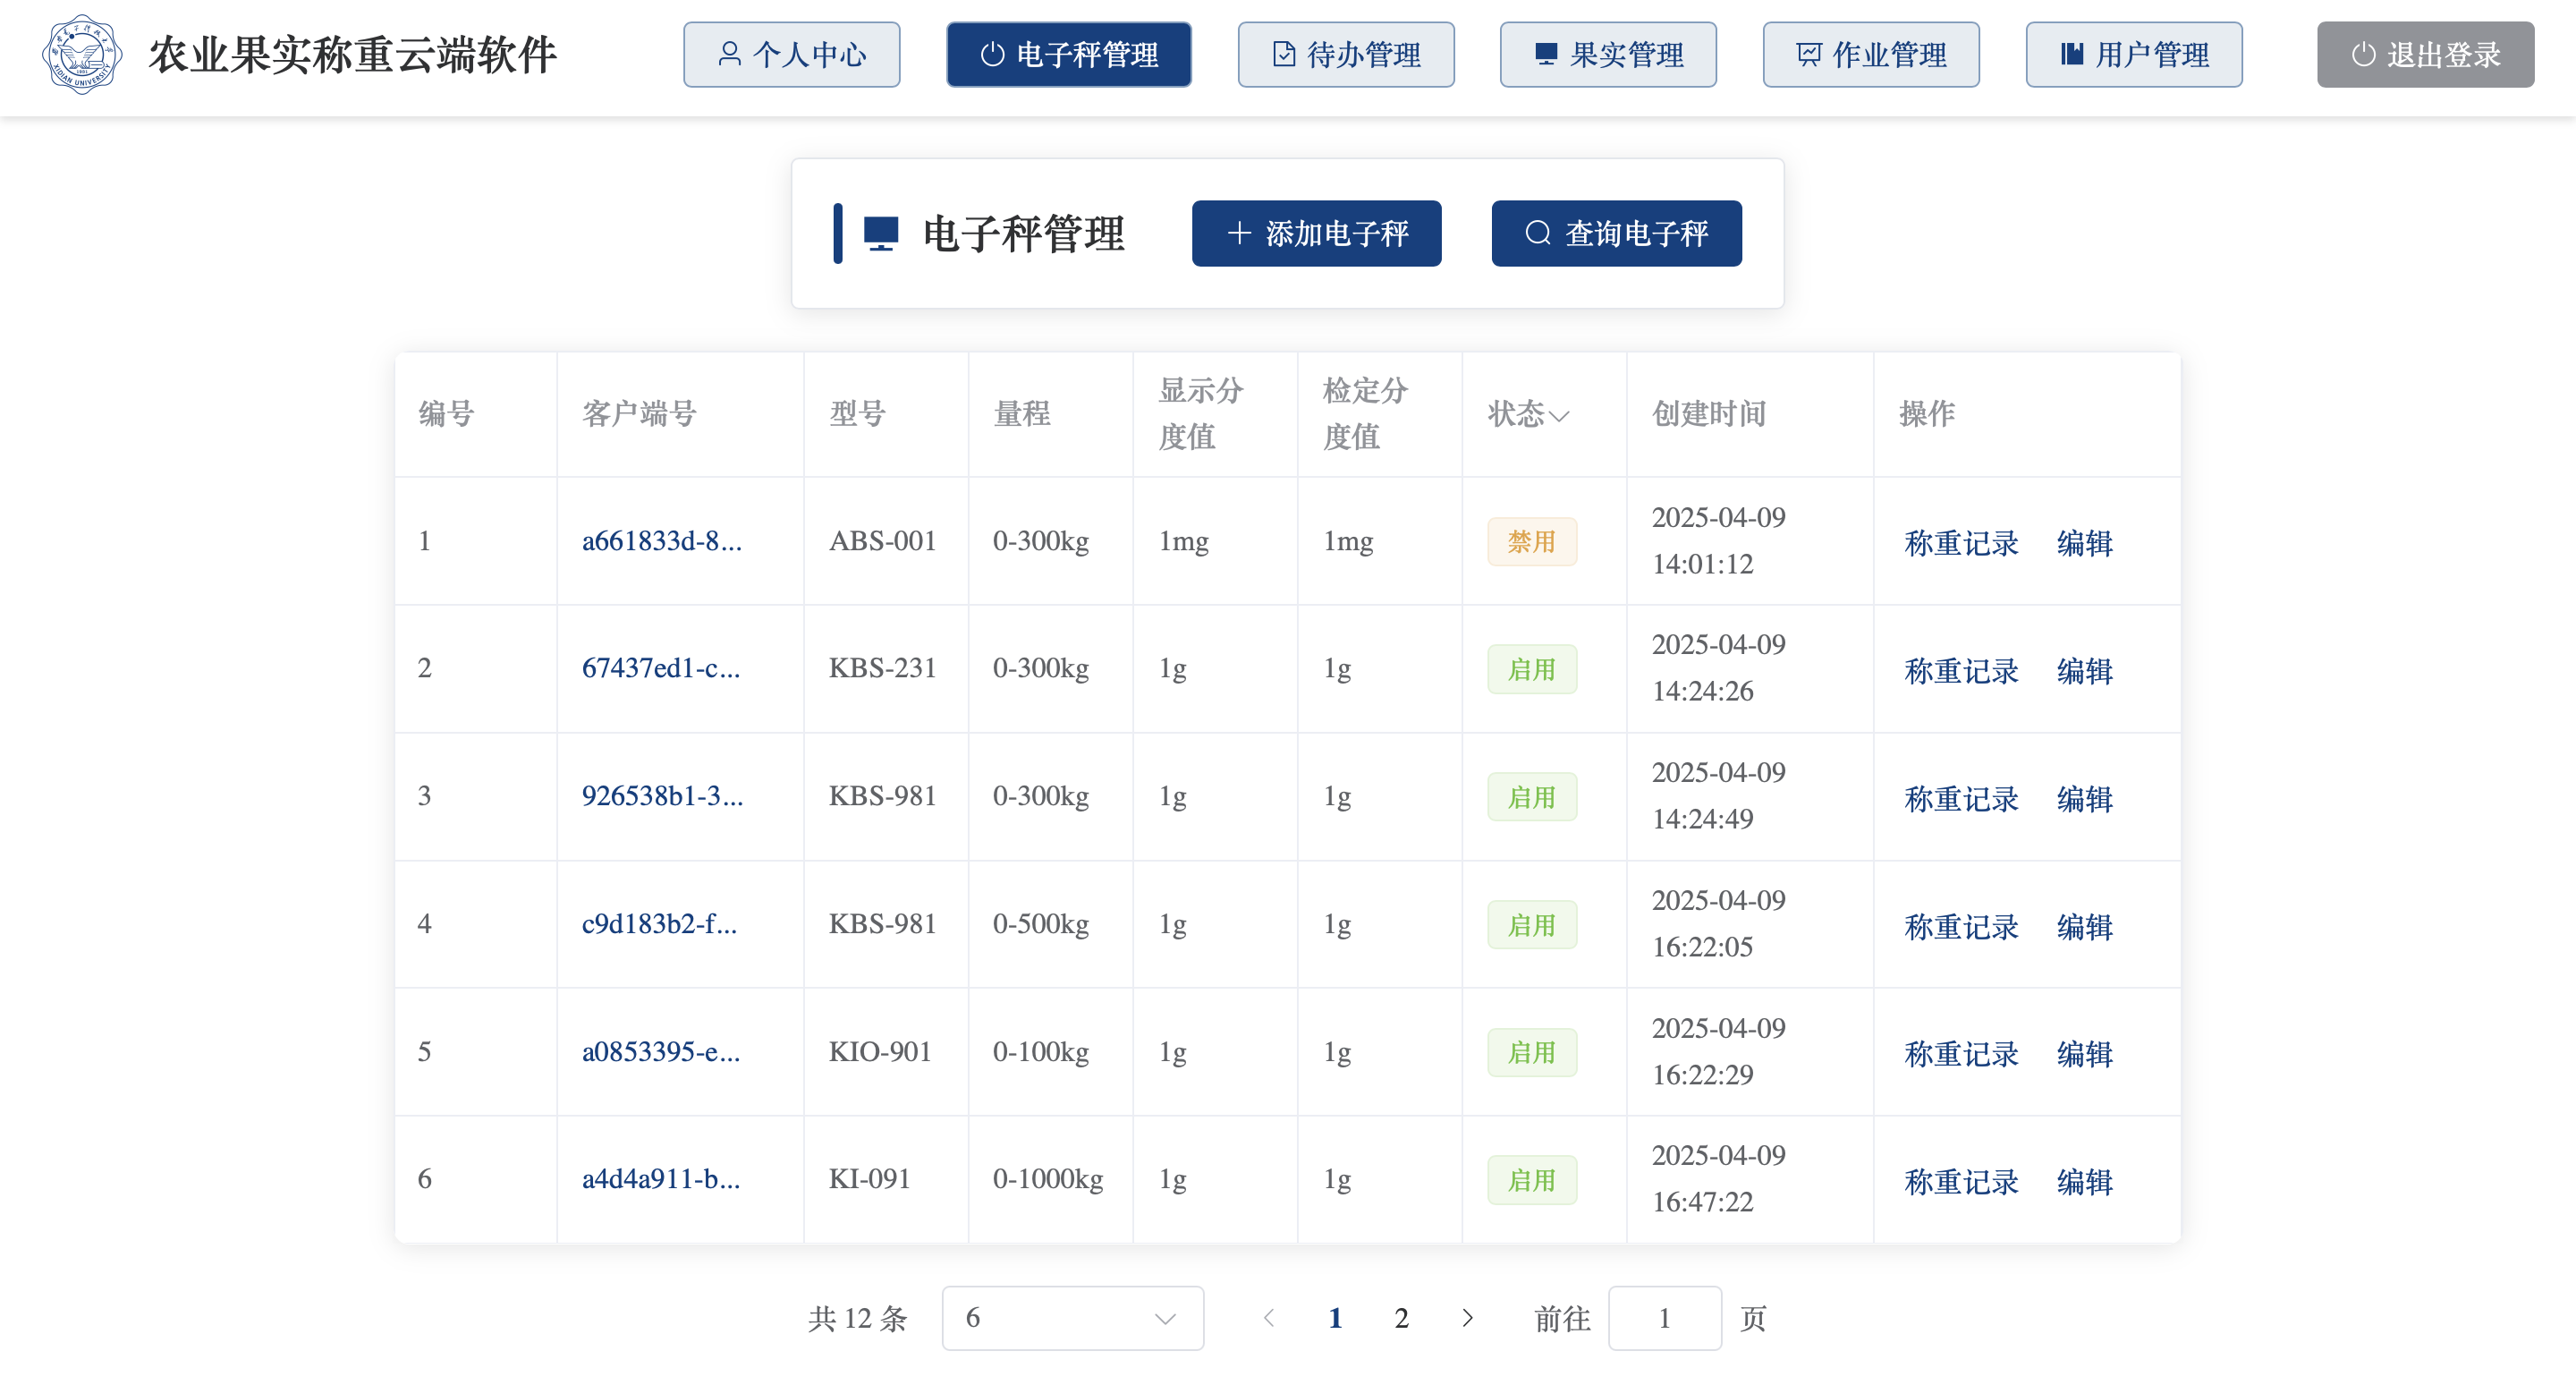
\includegraphics[width=0.9\linewidth]{../result/web-scale.png}
    \caption{电子秤管理界面}
    \label{fig:web-scale}
\end{figure}

\begin{figure}[H]
    \centering
    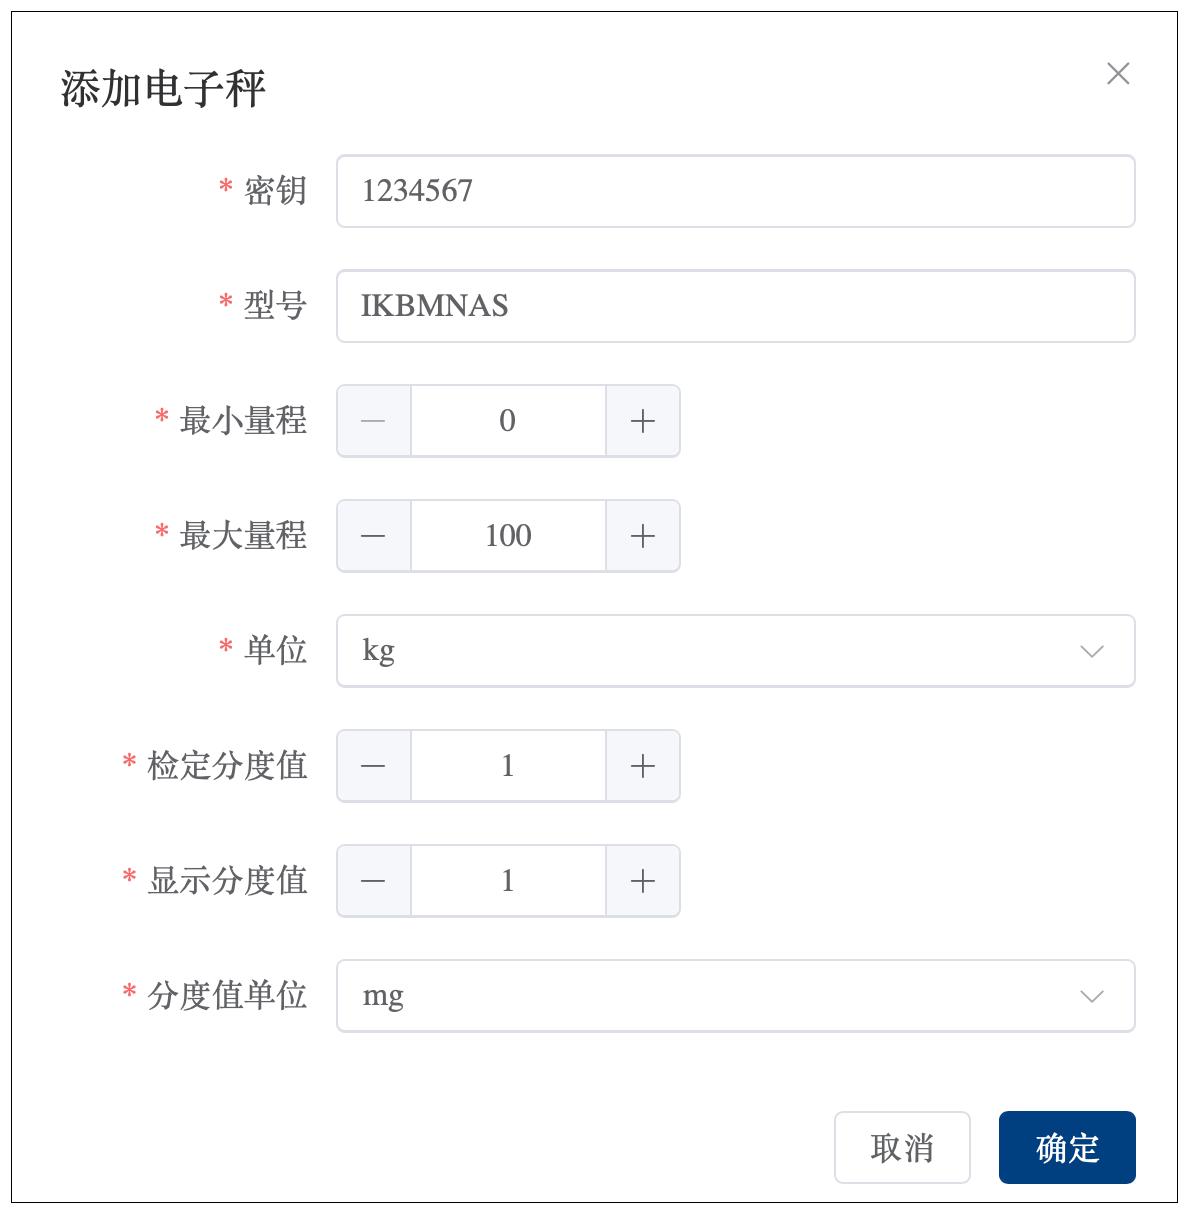
\includegraphics[width=0.9\linewidth]{../result/form-new-scale.png}
    \caption{电子秤配置表单}
    \label{fig:form-new-scale}
\end{figure}

图\ref{fig:web-scale}展现了软件管理后台中的电子秤管理界面,其中包含操作面板、电子秤列表和分页块。操作面板包含两个操作按钮,分别是添加电子秤和查询电子秤。电子秤列表中表头从左到右分别是编号、客户端号、型号、量程、显示分度值、检定分度值、状态、创建时间和支持的操作项,支持的操作项包含查看称重记录和编辑操作。

点击操作面板中的添加电子秤按钮,得到如图\ref{fig:form-new-scale}所显示的配置表单,表单项包含密钥、型号、最小最大量程及其单位、检定和显示分度值及其单位。

对用户认证和授权需求用例\ref{tab:uc-user-auth}设计测试用例并进行测试,如表\ref{tab:uc-user-auth-test}所示,采摘员工和管理员分别访问个人信息与用户列表接口,验证权限控制是否生效。普通用户访问被限制接口时返回 403,管理员访问全部接口均返回 200,结果符合预期。

\begin{table}[H]
    \centering
    \caption{用户认证和授权用例测试}
    \label{tab:uc-user-auth-test}
\begin{tblr}
    {
        colspec={Q[c,m]X[c,m]},
        hlines,vlines,cell{2-Z}{1}={},
        cell{1-Z}{1}={font=\bfseries},
        cell{1-Z}{2}={halign=l}
    }

用例名称 & 用户认证和授权 \\

用例描述 & 用户在后台管理界面中执行操作时的认证和授权流程 \\

用例入口 & 接口请求工具 Rest Client \\

测试步骤 & 步骤1. 调用登录接口获取到认证令牌 \newline
步骤2. 调用普通用户功能接口 \newline
步骤3. 调用管理员功能接口 \\

测试用例 & 用例1:采摘员工调用查看个人信息接口 \newline
用例2: 管理员调用查看个人信息接口 \newline
用例3: 采摘员工调用查看用户列表接口 \newline
用例4: 管理员调用查看用户列表接口 \\

预期结果与实际结果 & 用例1:预期返回数据和状态码 200,实际结果一致 \newline
用例2:预期返回数据和状态码 200,实际结果一致 \newline
用例3:预期返回错误信息和状态码 403,实际结果一致 \newline
用例4:预期返回数据和状态码 200,实际结果一致 \\
\end{tblr}
\end{table}

实际界面的测试情况如图\ref{fig:rest-user-auth-admin}和\ref{fig:rest-user-auth-emp}所示。

图\ref{fig:rest-user-auth-admin}展现了管理员调用接口的结果。首先调用用户登录接口获取到认证令牌;接着通过令牌调用查看个人信息接口,返回个人信息,其中用户角色显示为管理员(ROLE\_ADMIN),状态码为 200;最后调用查看用户列表接口,返回用户列表,状态码为200。结果符合预期,测试通过。

\begin{figure}[H]
    \centering
    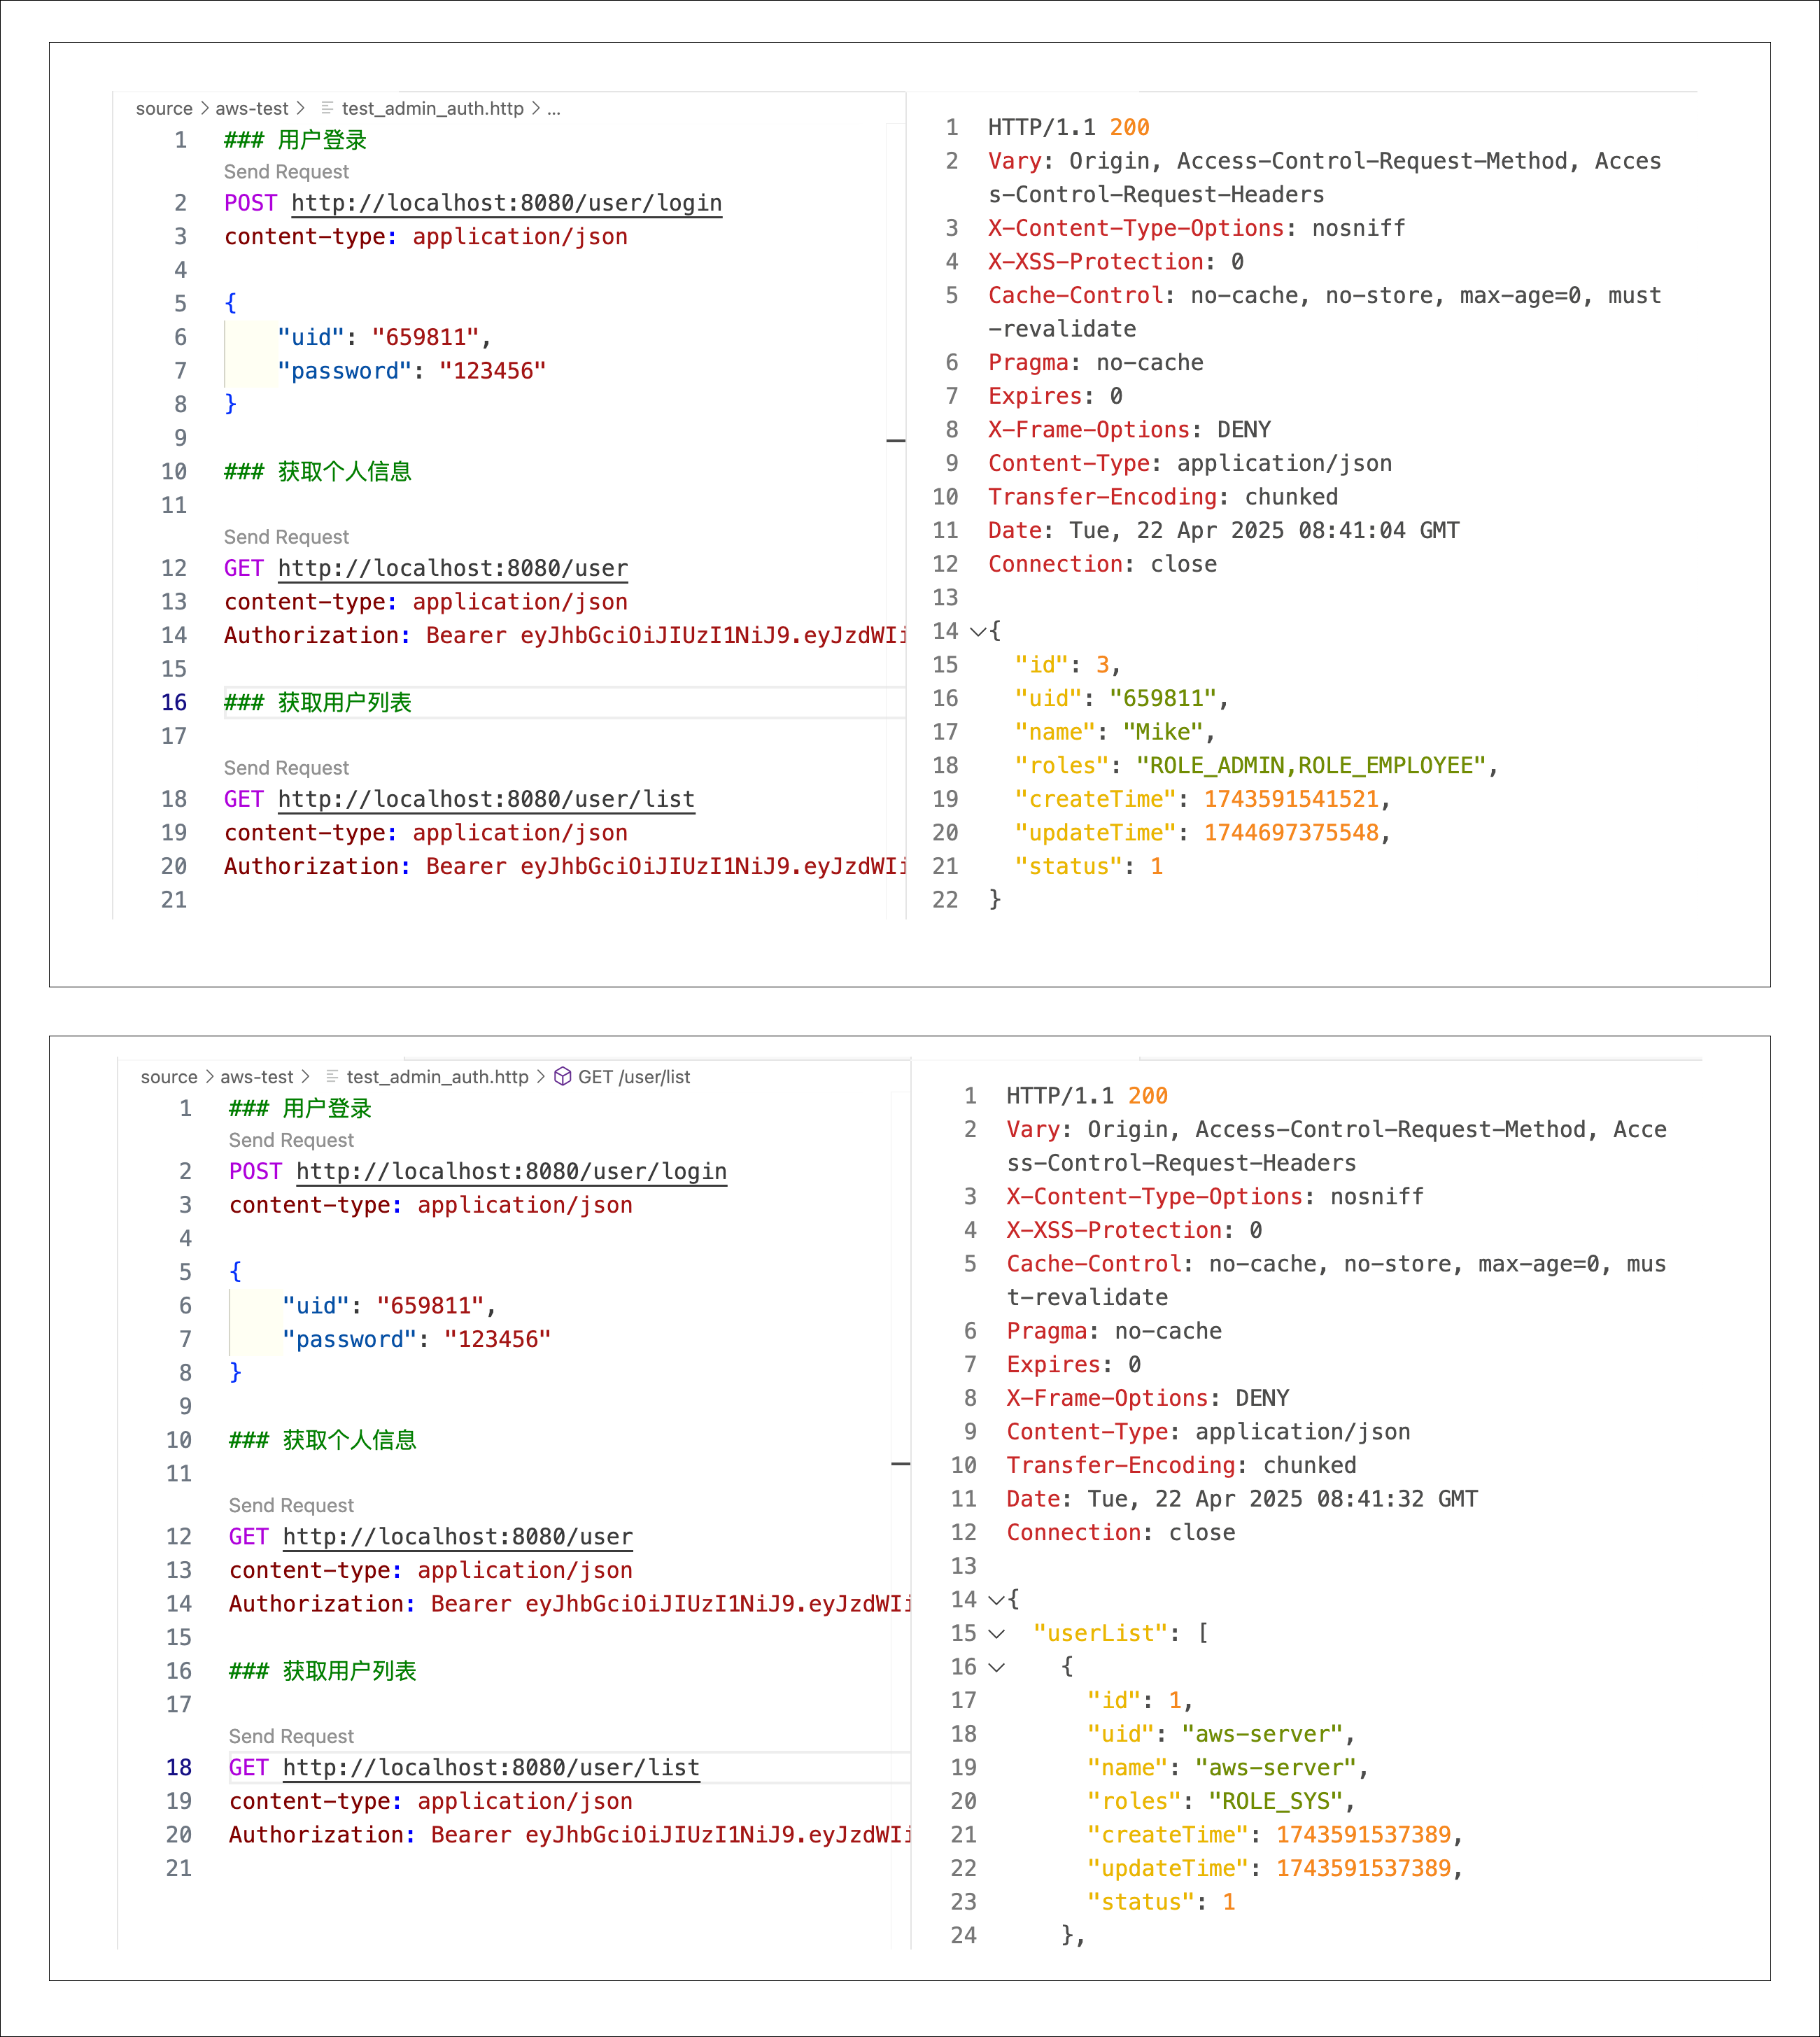
\includegraphics[width=0.9\linewidth]{../result/rest-user-auth-admin.png}
    \caption{管理员认证和授权接口测试}
    \label{fig:rest-user-auth-admin}
\end{figure}

图\ref{fig:rest-user-auth-emp}展现了采摘员工调用接口的结果。首先调用用户登录接口获取到认证令牌;接着通过令牌调用查看个人信息接口,返回个人信息,其中用户角色显示为采摘员工(ROLE\_EMPLOYEE),状态码为 200;最后调用查看用户列表接口,返回 Access Denied(访问拒绝),状态码为 403。结果符合预期,测试通过。

\begin{figure}[H]
    \centering
    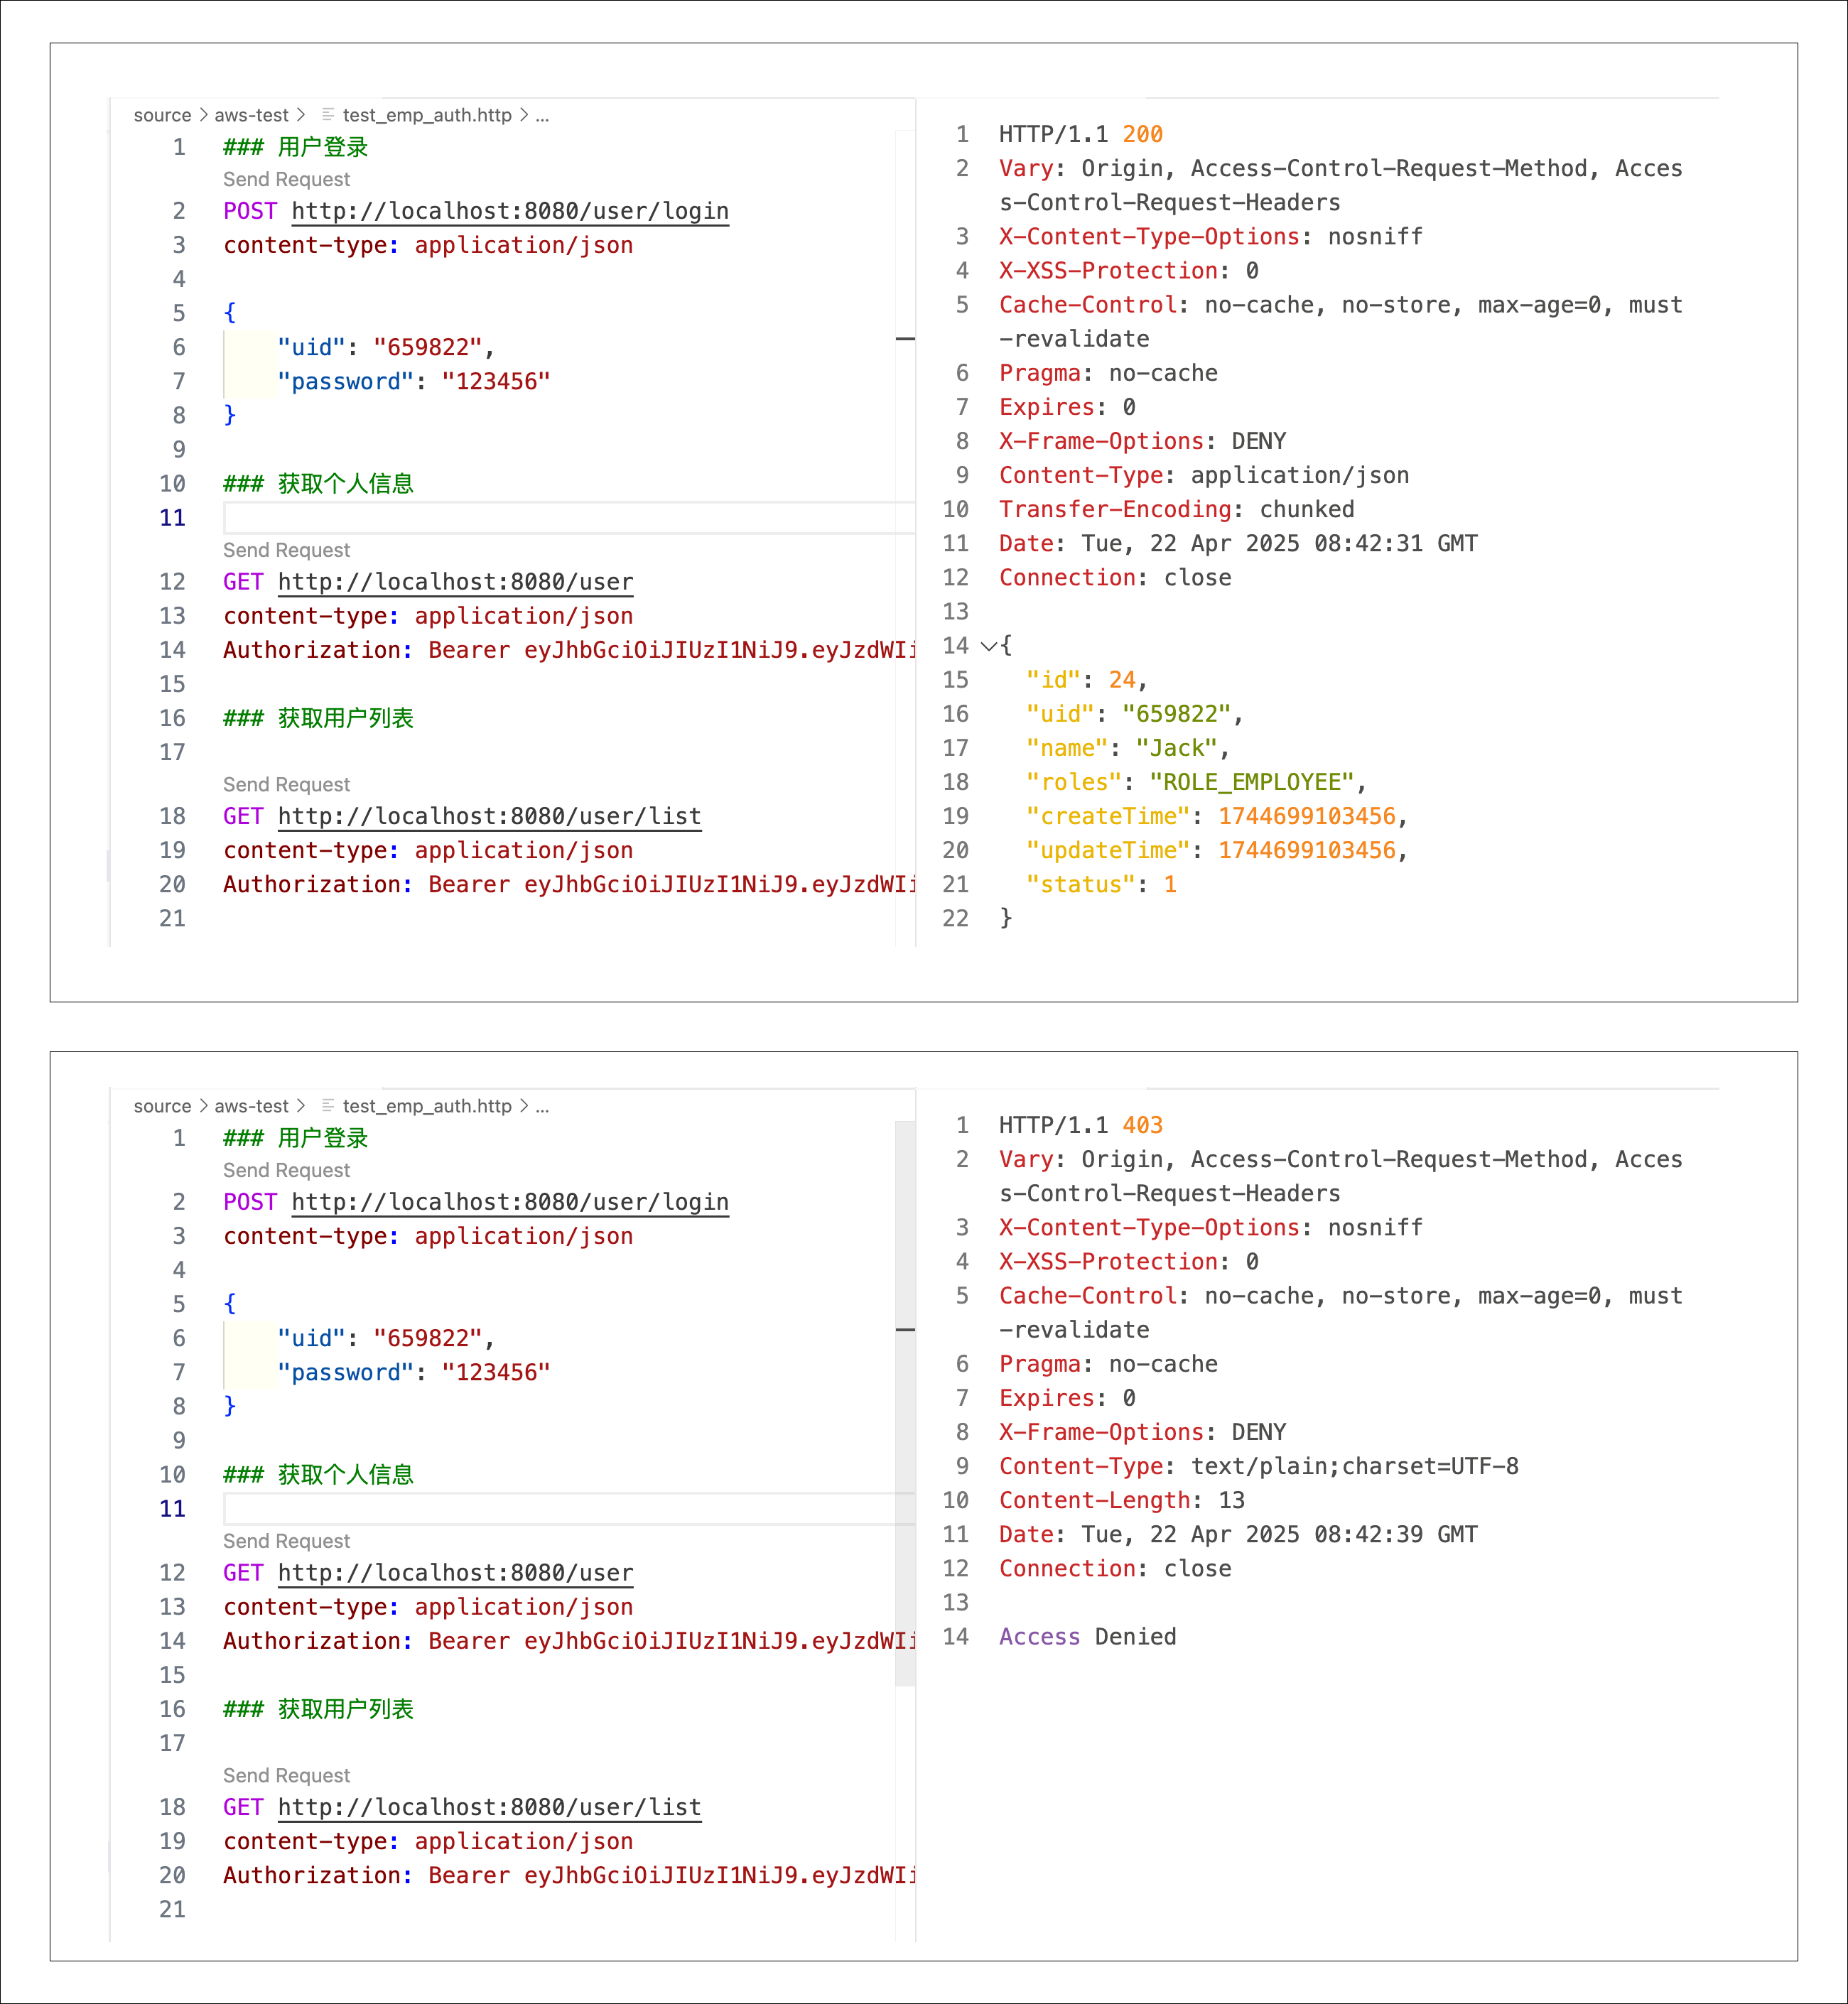
\includegraphics[width=0.9\linewidth]{../result/rest-user-auth-emp.png}
    \caption{采摘员工认证和授权接口测试}
    \label{fig:rest-user-auth-emp}
\end{figure}

对果实图像识别需求用例\ref{tab:uc-produce-predict}设计测试用例并进行测试,如表\ref{tab:uc-produce-predict-test}所示,提交支持的果实图像(如苹果)时,模型成功识别且结果正确;提交不支持的果实图像(如火龙果)时,预测失败,预期与实际一致。

\begin{table}[H]
    \centering
    \caption{果实图像识别用例测试}
    \label{tab:uc-produce-predict-test}
\begin{tblr}
    {
        colspec={Q[c,m]X[c,m]},
        hlines,vlines,cell{2-Z}{1}={},
        cell{1-Z}{1}={font=\bfseries},
        cell{1-Z}{2}={halign=l}
    }
用例名称 & 果实图像识别用例 \\

用例描述 & 调用本地模型推理预测果实种类 \\

用例入口 & 接口请求工具 Rest Client \\

测试步骤 & 步骤1. 输入果实图片地址 \newline
步骤2. 调用果实图像识别接口 \\

测试用例 & 用例1:提交模型支持的果实图片(苹果) \newline
用例2: 提交模型不支持的果实图片(火龙果) \\

预期结果与实际结果 & 用例1:预期为成功预测果实种类为苹果,实际结果一致 \newline
用例2:预期为预测失败,实际结果一致 \\

\end{tblr}
\end{table}

实际界面的测试情况如图\ref{fig:rest-produce-predict}所示,图中上方请求提交了苹果图片,返回结果中得到预测置信度排名第一位的果实为苹果,置信度为 0.93563,符合预期;下方请求显示提交了火龙果图片,返回结果为空,预测失败,符合预期。

\begin{figure}[H]
    \centering
    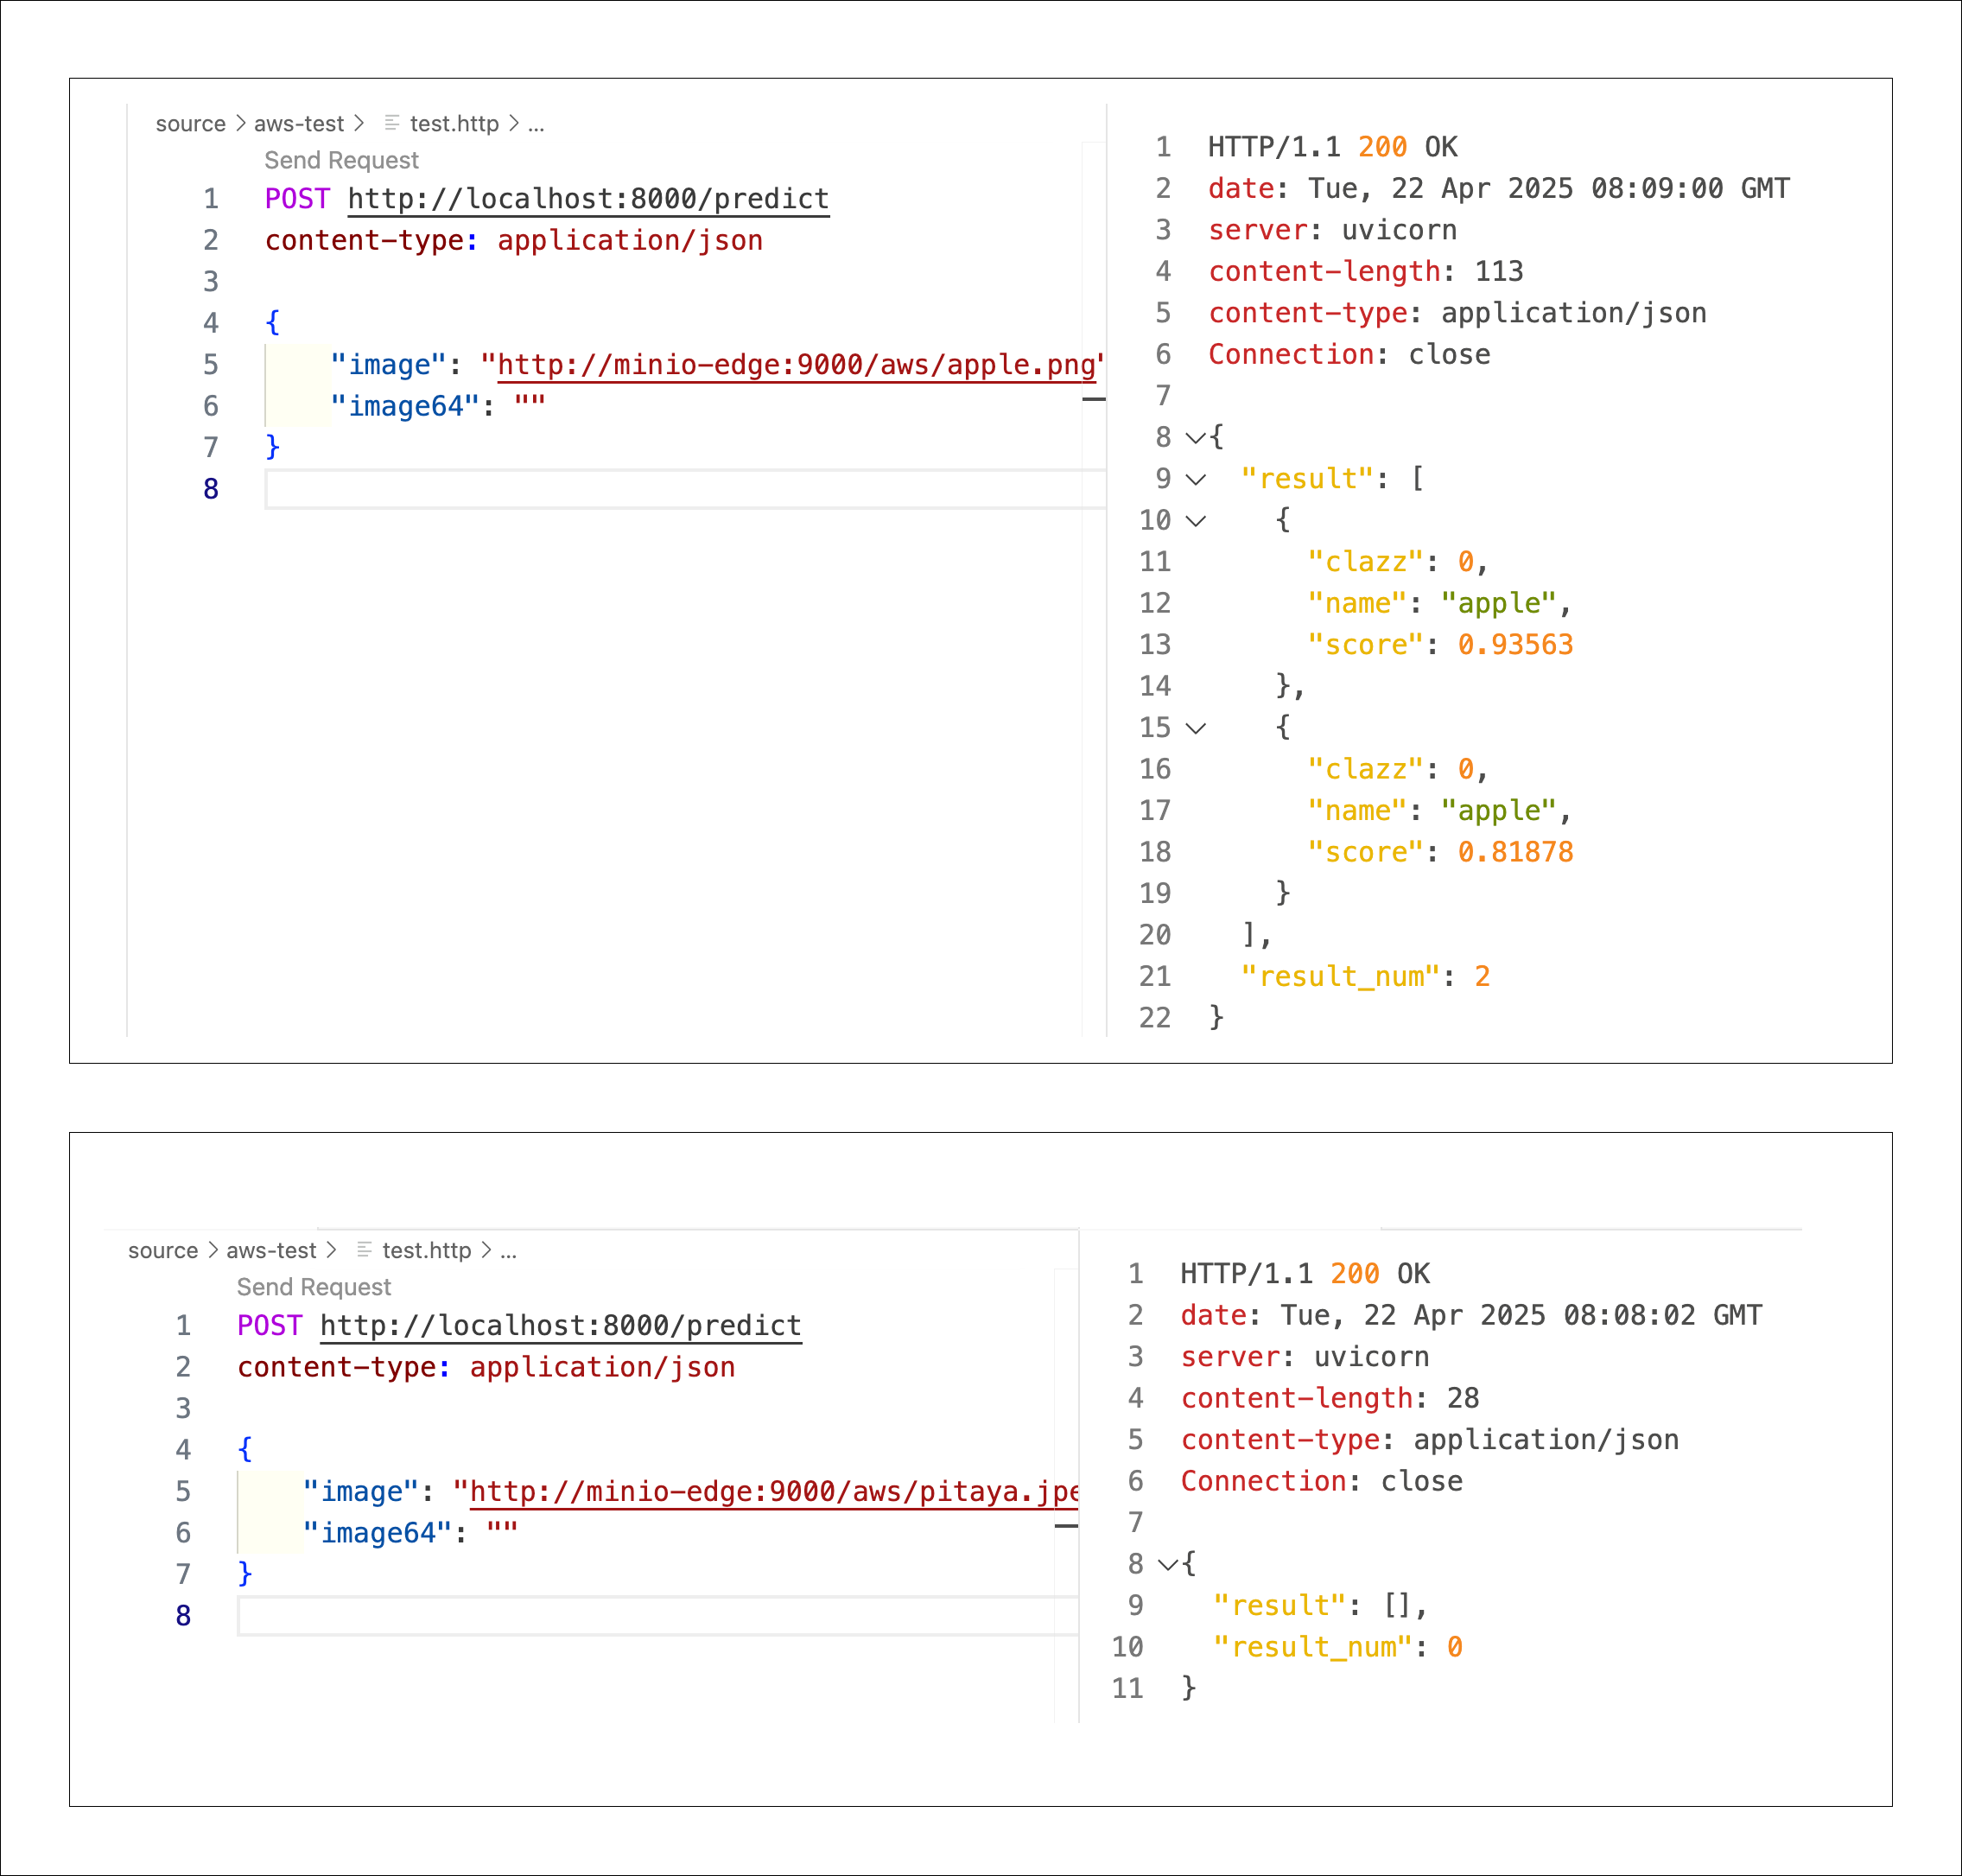
\includegraphics[width=0.9\linewidth]{../result/rest-produce-predict.png}
    \caption{果实图像识别接口测试}
    \label{fig:rest-produce-predict}
\end{figure}

对新建采摘作业需求用例\ref{tab:uc-work-new}设计测试用例并进行测试,如表\ref{tab:uc-work-new-test}所示,选择启用的果实(如苹果)时创建成功;选择未启用的果实(如香蕉)或已有作业的果实时创建失败,实际结果与预期一致。

\begin{table}[H]
    \centering
    \caption{新建采摘作业接口测试}
    \label{tab:uc-work-new-test}
\begin{tblr}
    {
        colspec={Q[c,m]X[c,m]},
        hlines,vlines,cell{2-Z}{1}={},
        cell{1-Z}{1}={font=\bfseries},
        cell{1-Z}{2}={halign=l}
    }

用例名称 & 新建采摘作业用例 \\

用例描述 & 对某一果实新建对于采摘作业 \\

用例入口 & 后台管理界面中的作业管理模块 \\

测试步骤 & 步骤1. 点击添加作业 \newline
步骤2. 选择采摘产品 \newline
步骤3. 选择起止时间 \newline
步骤4. 点击确认完成添加 \\

测试用例 & 用例1: 提交正常数据(选择已启用的果实:苹果) \newline
用例2: 提交异常数据(选择未启用的果实:香蕉) \newline
用例3: 提交异常数据(选择已有对应采摘作业的果实:苹果) \\

预期结果与实际结果 & 用例1:预期返回"成功",实际结果一致 \newline
用例2:预期返回"失败",实际结果一致 \newline
用例3:预期返回"失败",实际结果一致 \\

\end{tblr}
\end{table}

实际界面的测试情况如图\ref{fig:web-work}和图\ref{fig:form-new-work}所示。

图\ref{fig:web-work}展现了软件管理后台中的作业管理界面,其中包含作业列表、4个操作按钮和分页块,其中作业列表表头包含编号、采摘产品、开始时间、结束时间、采摘量、状态和操作;操作按钮包含添加作业、查询作业、导出作业数据和编辑。点击添加作业按钮后,显示表单如图\ref{fig:form-new-work}所示。

\begin{figure}[H]
    \centering
    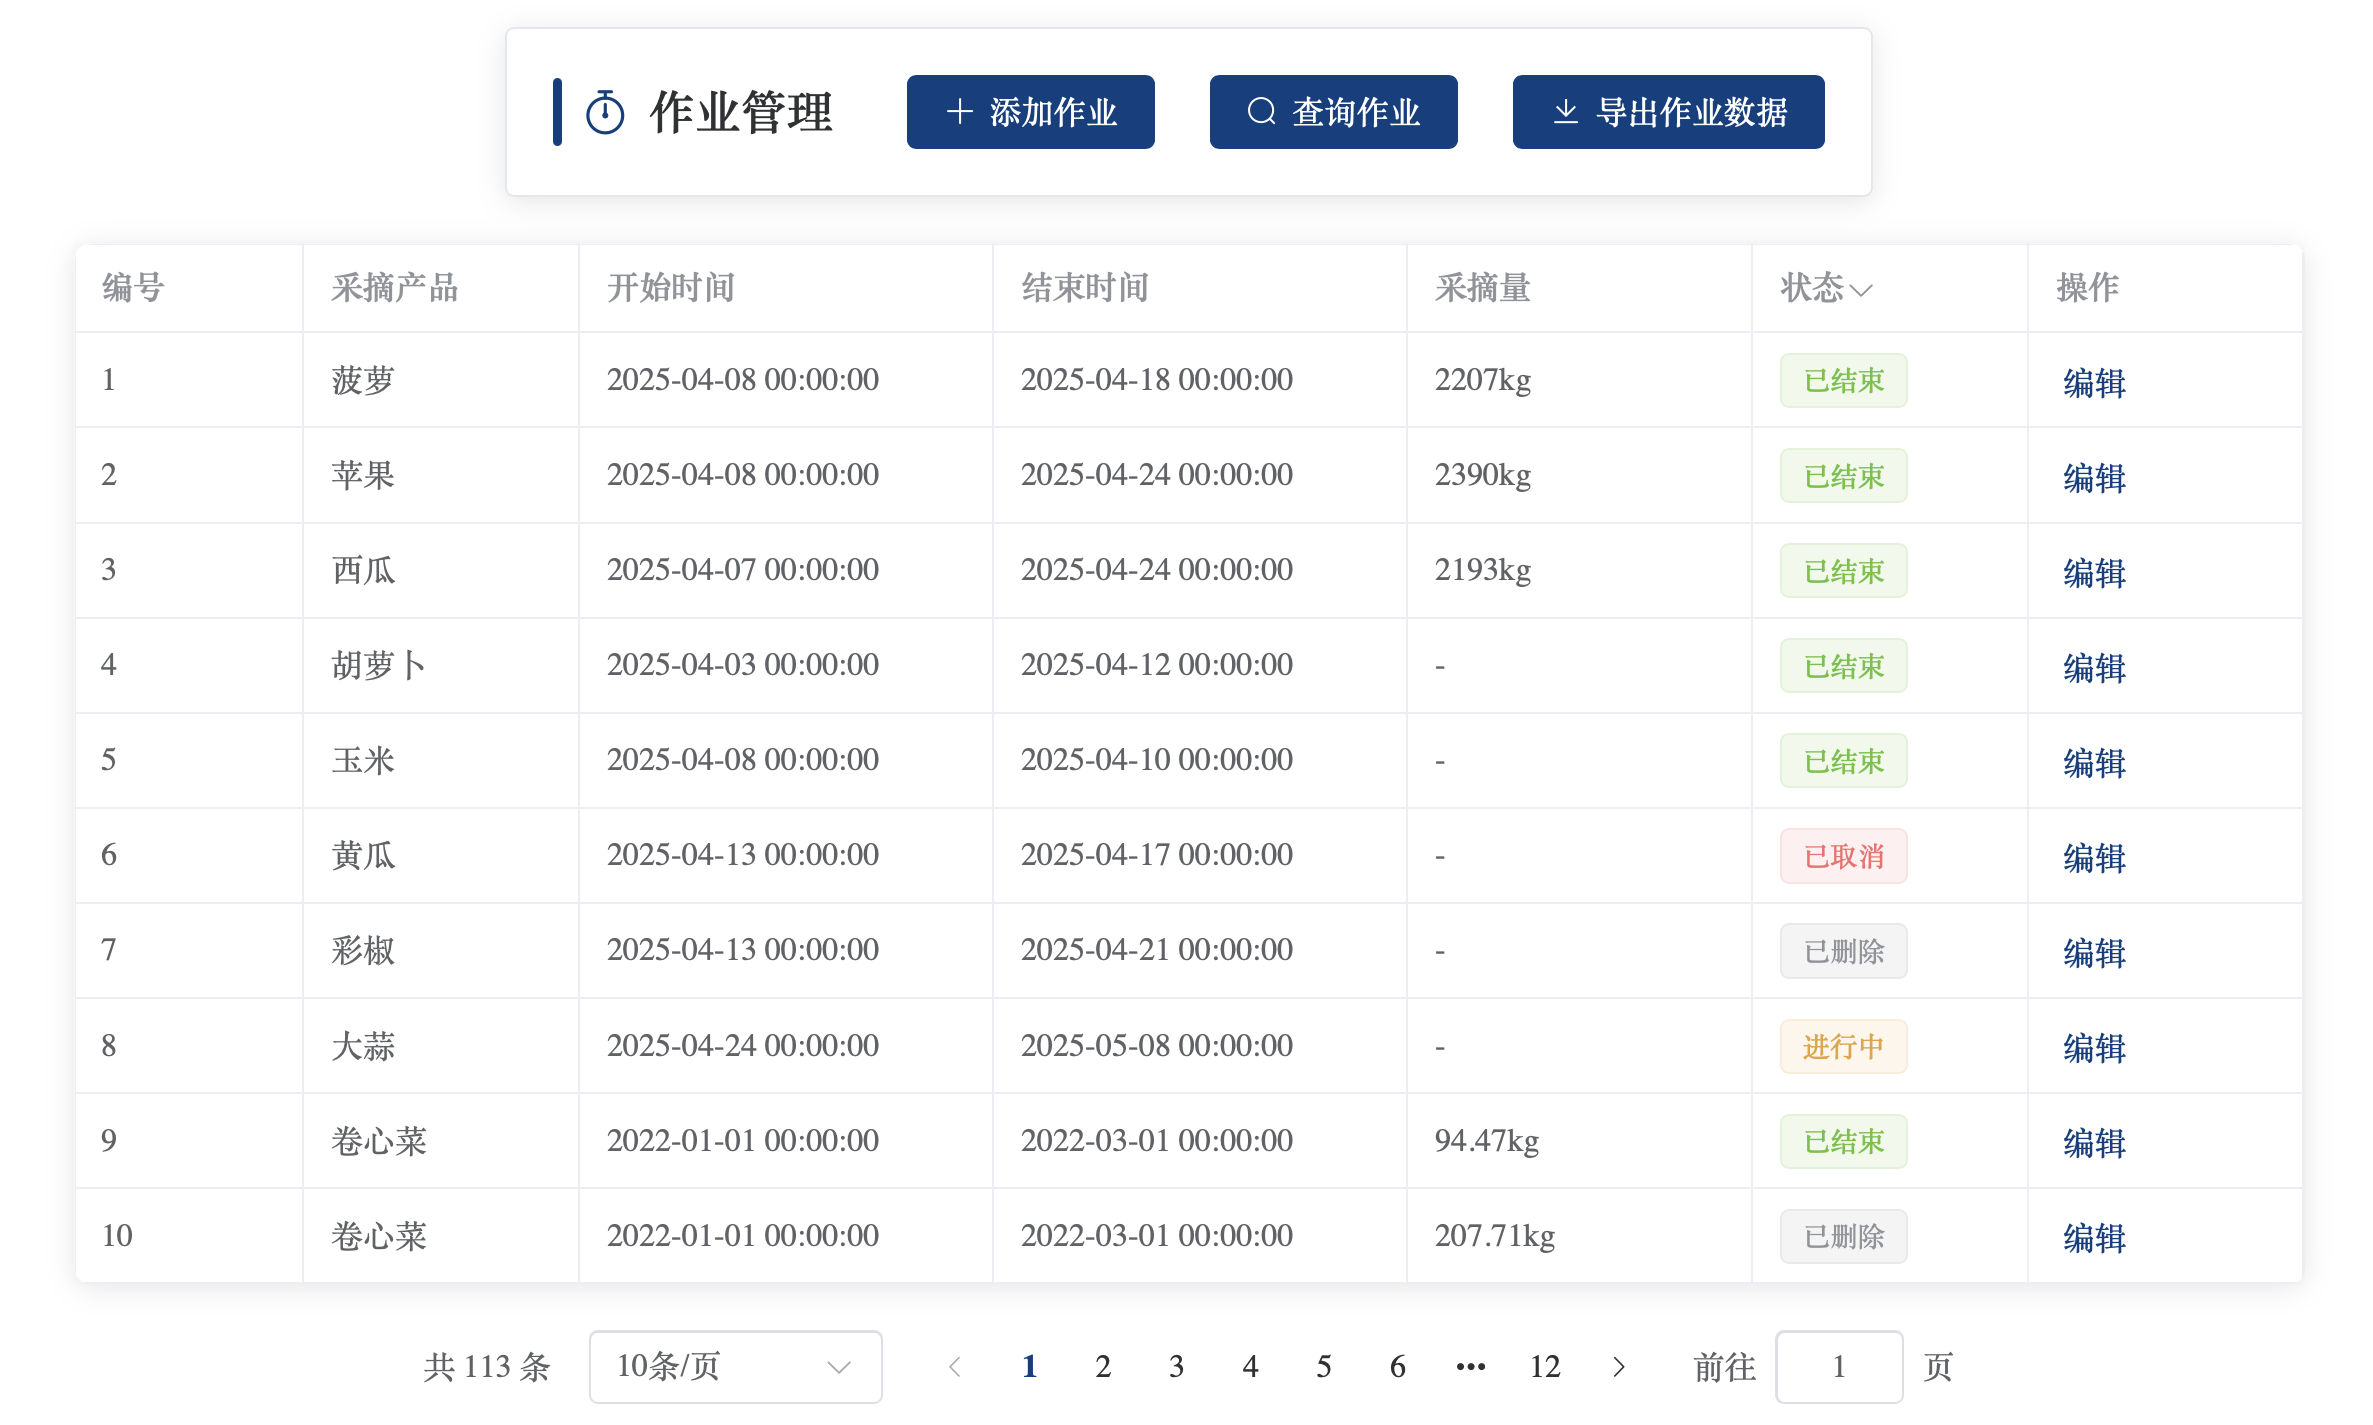
\includegraphics[width=0.9\linewidth]{../result/web-work.png}
    \caption{采摘作业管理界面}
    \label{fig:web-work}
\end{figure}

图\ref{fig:form-new-work}展现了作业项的提交表单,包含2个操作按钮和3个表单项,其中操作按钮包含取消和确认按钮;表单项包含选择采摘产品、开始时间和结束时间,采摘产品在下滑表单中选择,开始时间和结束时间点击后在日历组件中选择。

\begin{figure}[H]
    \centering
    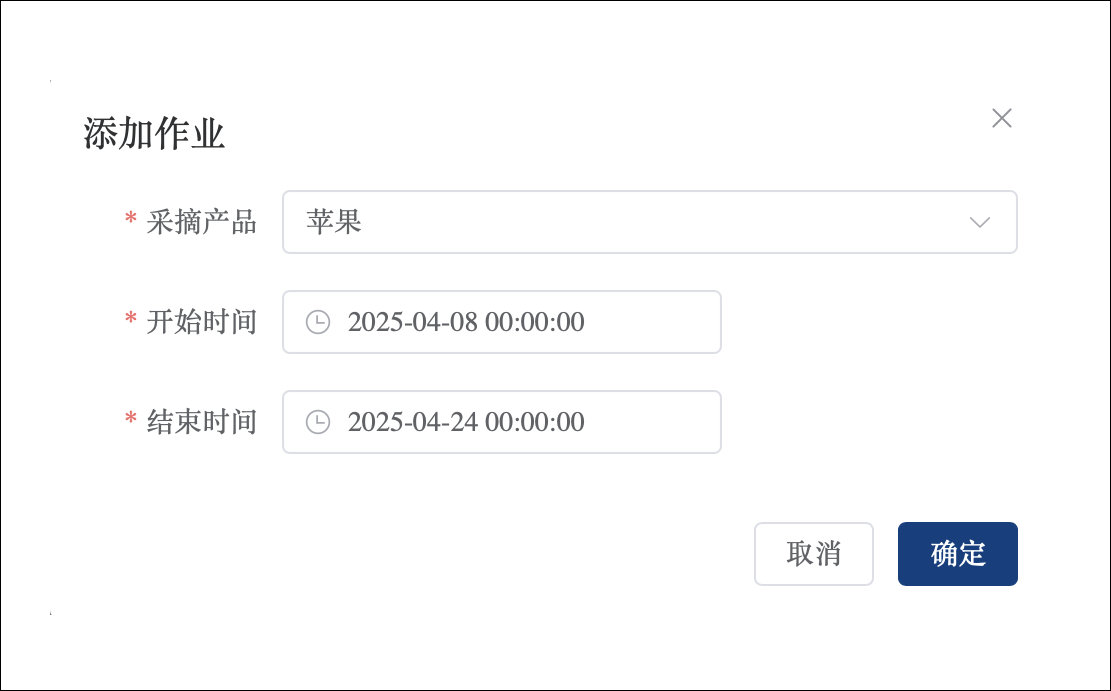
\includegraphics[width=0.9\linewidth]{../result/form-new-work.png}
    \caption{新建采摘作业表单}
    \label{fig:form-new-work}
\end{figure}

\section{软件性能测试}

根据非功能需求汇总表\ref{tab:n-req-summary}中提到的功能,给出对应的实现结果,如表\ref{tab:test-n-req-summary}所示。本节针对提供高性能服务这个非功能需求,下面给出软件具体的性能测试和分析结果。首先给出对果实图像识别服务的性能测试,然后再给出称重数据提交服务的性能测试。

\begin{table}[H]
    \centering
    \caption{非功能需求实现结果}
    \label{tab:test-n-req-summary}
\begin{tblr}
    {
    colspec        = {Q[c,m]X[l,m]},
    hline{1,Z}     = {wd=.08em},
    hline{2}       = {wd=.05em},
    row{even[2-Z]} = {bg=gray9!50},
    row{1}         = {font=\bfseries},
    rowhead        = 1,
    }
测试项 & 描述 & 测试结果 \\
支持多种协议 & 支持 MQTT、HTTP、CoAP、STOMP 四种协议 & 验证通过 \\
支持多种提交方式 & 支持通过果实图像/名称/编号提交称重数据 & 验证通过 \\
支持模拟提交流程 & 支持通过电子秤模拟器模拟数据提交 & 验证通过 \\
支持受限网络环境 & 支持在边端提交数据 & 验证通过 \\
提供高性能的服务 & 提供高性能的果实图像识别服务和称重数据提交服务 & 验证通过 \\
提供安全性保障 & 数据库加密敏感字段,所有接口提供认证授权保护 & 验证通过 \\
\end{tblr}
\end{table}

下面对训练出来的果实图像识别模型进行性能测试。

(1)测试环境:4 核 CPU, 31.4GB 内存, 2 个 Tesla T4 GPU。

(2)测试方式:使用 Ultralytics 提供的性能测试库,调用训练出来的最佳模型 best.pt,测试数据则采用训练集数据。

(3)测试结果:如图 \ref{fig:model-benchmark} 所示。

\begin{figure}[H]
    \centering
    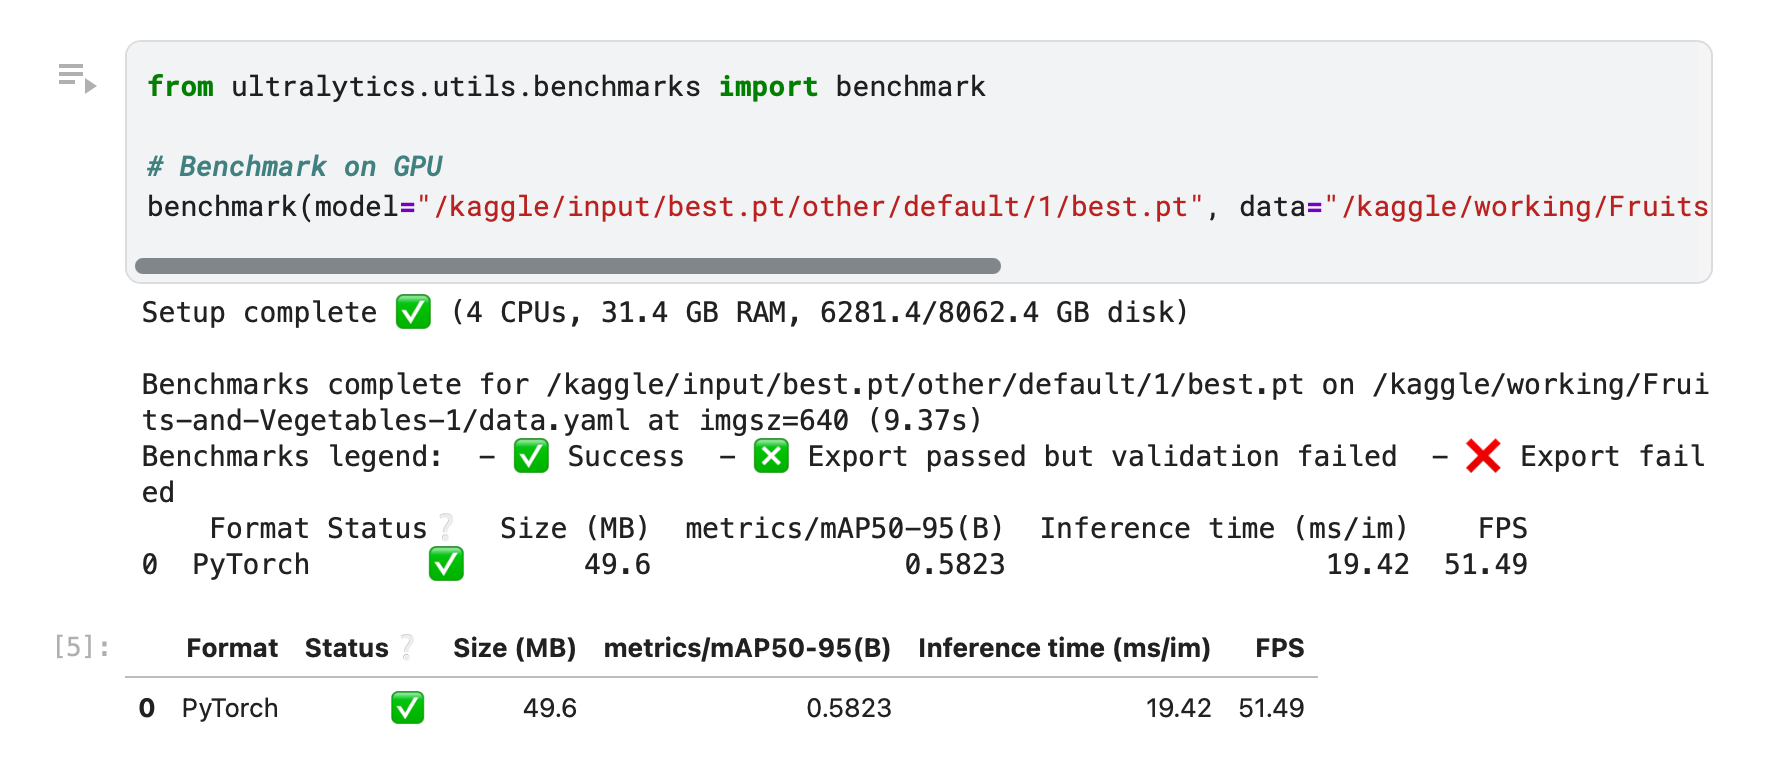
\includegraphics[width=0.95\linewidth]{../source/aws-img/yolov8/benchmark.png}
    \caption{果实图像识别模型性能测试结果}
    \label{fig:model-benchmark}
\end{figure}

从图 \ref{fig:model-benchmark} 可以得出,模型使用 PyTorch 框架训练,推理时间为 19.42 毫秒,帧率为 51.49 FPS,且在 mAP50-95 指标下的得分为 0.5823,适用于精度和推理速度之间的平衡。

训练模型得到标准化混淆矩阵图\ref{fig:confusion_matrix_normalized},图中的标准化混淆矩阵可以看出,模型在多个类别上表现出色。例如,apple(苹果)、banana(香蕉) 和 carrot(胡萝卜) 等类别的预测准确率都超过了 90\%。然而,某些类别的分类效果较差,chilli\_pepper(辣椒)的准确率为 62\%,并且容易被误分类为 corn(玉米) 或其他类别。总体来说,模型在多数类别上的表现良好,大部分类别的置信度都在 0.7 到 1.0 之间。

\begin{figure}
    \centering
    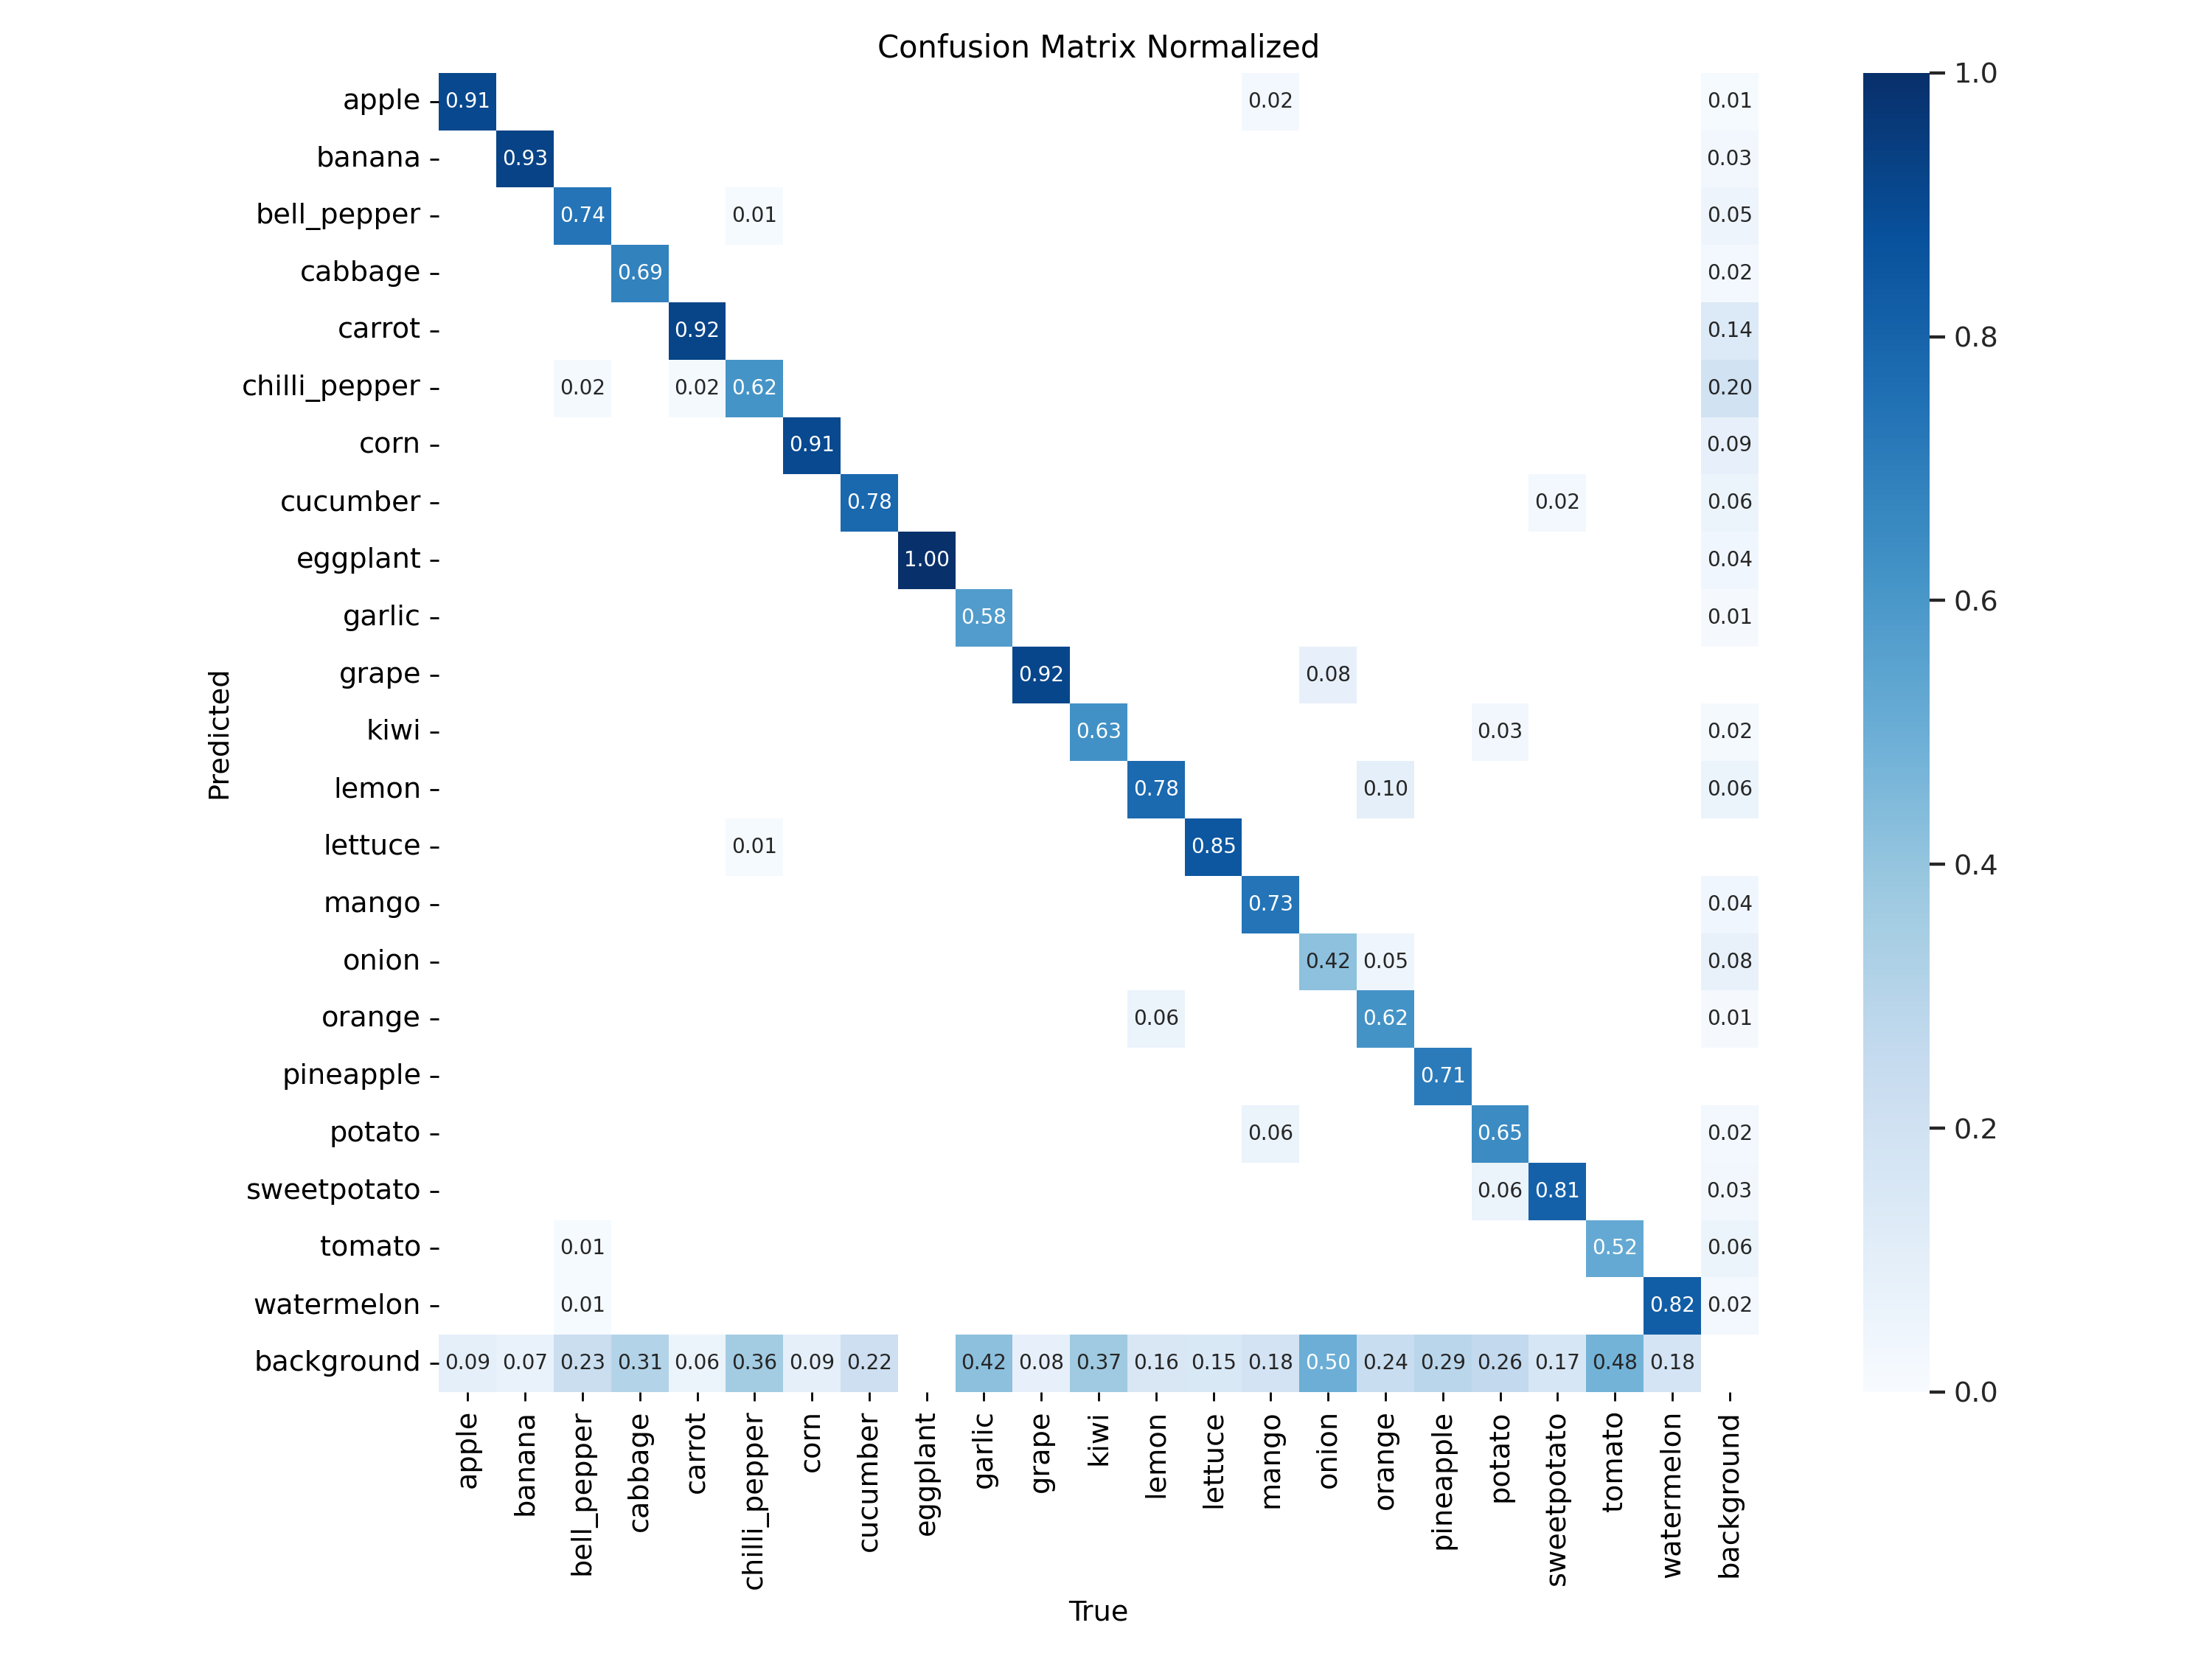
\includegraphics[width=0.95\linewidth]{../source/aws-img/yolov8/out/image/confusion_matrix_normalized.png}
    \caption{果实图像识别模型训练结果-标准化混淆矩阵图}
    \label{fig:confusion_matrix_normalized}
\end{figure}

综上所述,训练出来的果实图像识别模型在精度与推理速度之间达到平衡,模型在多数类别上的识别效果表现良好。

对于称重数据的提交,下面根据压力测试的方法\cite{Zhu2017}来对其进行性能测试,通过测试软件 JMeter 模拟 HTTP 并发请求来统计各项性能指标:

(1)测试环境:8 核 CPU, 8GB 内存 的 Docker 容器。

(2)测试方式:启动称重相关服务,包含 Spring 应用服务、EMQX 集群以及MySQL 数据库服务,分别以并发数 100、200 和 500 对提交称重数据接口进行测试,Ramp-up Time(负载增长时间) 设为 30s,Hold Time(稳定负载时间)设为 35s。

(3)测试结果:如图\ref{fig:jmeter-test-result}所示。

\begin{figure}[H]
    \centering
    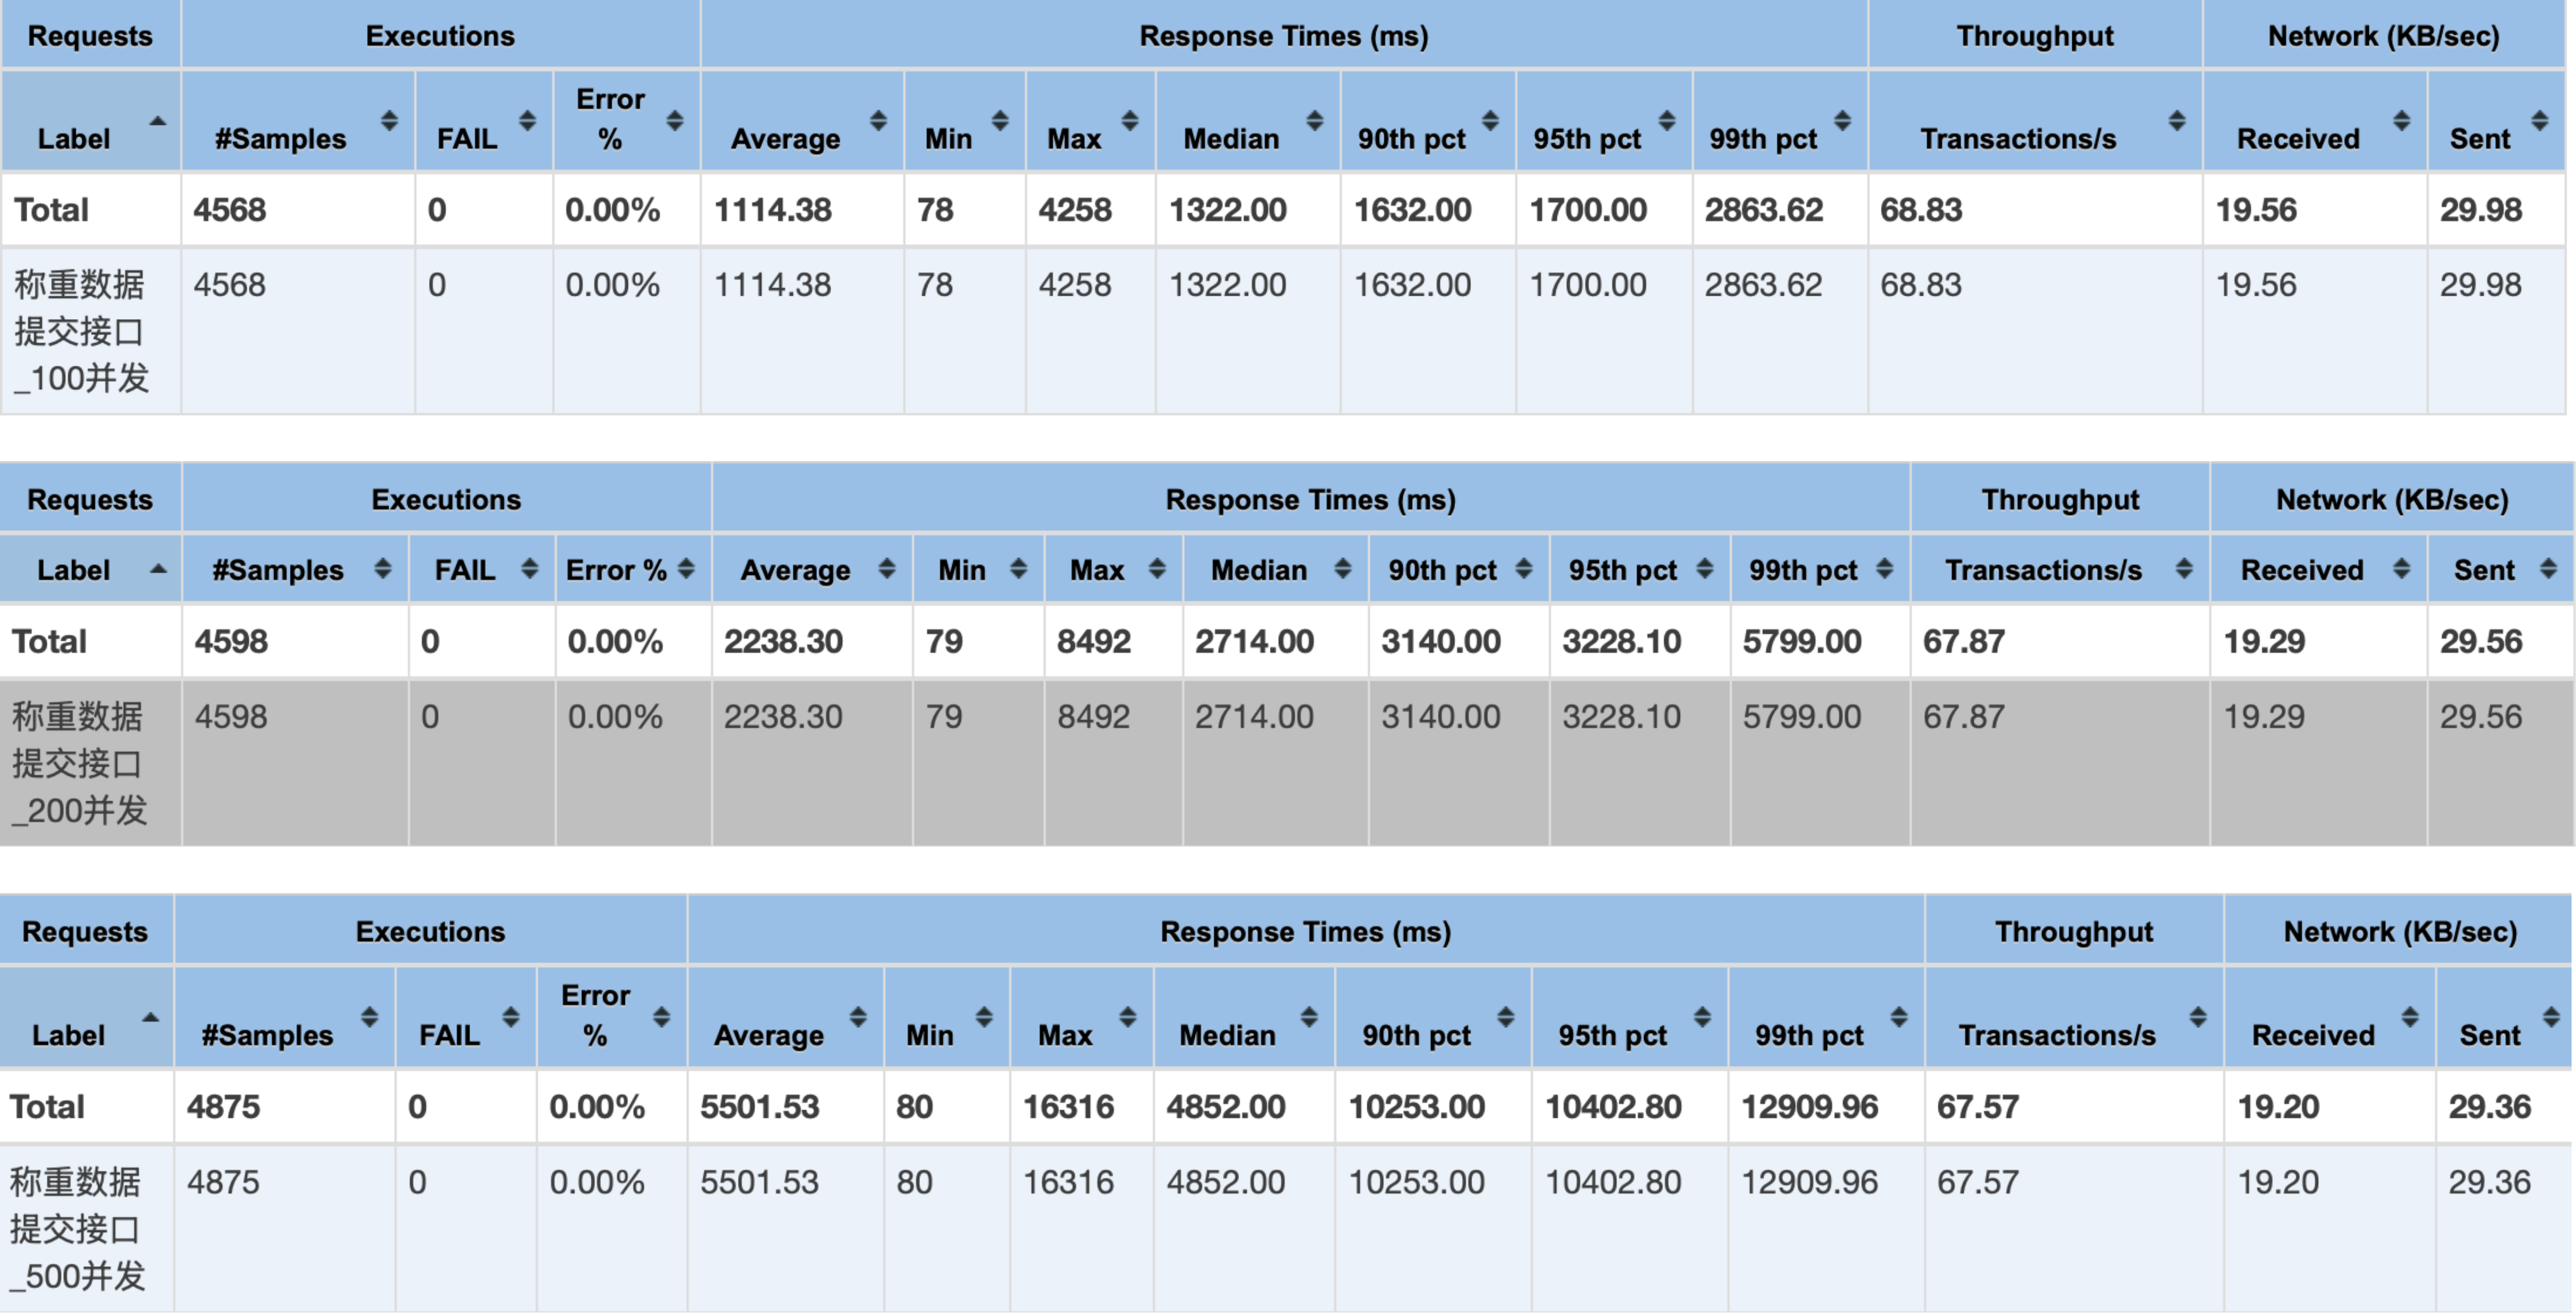
\includegraphics[width=0.95\linewidth]{../source/aws-test/jmeter-test-result.png}
    \caption{核心接口的压力测试结果}
    \label{fig:jmeter-test-result}
\end{figure}

图\ref{fig:jmeter-test-result}从上至下显示了并发数为 100、200 和 500 下的压力测试结果表格,每个表格从左至右显示的条目分别是测试标题、样本数、失败数、错误率、平均响应时间、最小响应时间、最大响应时间、响应时间中位数、90\%响应时间、95\%响应时间、99\%响应时间、吞吐量、网络接收数据量、网络发送数据量。

在 100 并发下,软件性能表现较好,响应时间在 1 秒内,大部分请求能够在合理时间内完成,吞吐量也较为稳定。此时软件能够处理较高的负载;在 200 并发下,响应时间明显增加,超过了 2 秒,并且最大响应时间接近 9 秒。吞吐量略有下降,软件开始在中等负载下显现出性能下降的迹象。虽然软件能够处理较高并发,但开始显示出压力;在 500 并发下,性能显著下降,平均响应时间超过了 5 秒,最大响应时间接近 16 秒,90\% 的请求响应时间超过 10 秒。吞吐量保持不变或略微下降,说明软件在高负载下的性能有严重瓶颈,无法有效处理 500 并发请求。此时软件可能面临资源瓶颈。

从上述分析可以知道,在 8 核 CPU, 8GB 内存的硬件条件下,软件可以高效地处理超过 200 台电子秤的并发请求,适合于中小型农场的部署使用。如果将并发数提高到 500,可以考虑升级硬件资源。

\section{本章小结}

本章详细介绍了软件测试与分析的过程和结果。首先给出了软件的测试环境,包括硬件配置和基于Docker Compose的容器化部署方案。在功能测试部分,针对需求分析阶段定义的核心功能用例进行了全面测试,包括电子秤管理、果实管理、作业管理、用户管理、称重记录处理、统计分析等模块,所有功能均通过测试并展示了相关界面截图和测试数据。性能测试部分重点评估了果实图像识别模型和称重数据提交接口的性能表现:YOLOv8模型在测试集上达到了0.5823的mAP50-95指标,推理速度为51.49FPS;称重数据接口在200并发下保持稳定,吞吐量达到预期水平。测试结果表明,系统各项功能和非功能需求均已实现,在精度和性能方面达到了设计目标,能够满足中小型农场的使用需求。
